% This example is meant to be compiled with lualatex or xelatex
% The theme itself also supports pdflatex
\PassOptionsToPackage{unicode}{hyperref}
\documentclass[aspectratio=1610, 10pt]{beamer}

% Load packages you need here
\usepackage[ngerman, english]{babel}

\usepackage[autostyle]{csquotes}

\usepackage{amsmath}
\usepackage{amssymb}
\usepackage{mathtools}
%%%% $Id: lhcb-symbols-def.tex 124462 2018-11-07 12:32:50Z pkoppenb $
%%% ======================================================================
%%% Purpose: Standard LHCb aliases
%%% Author: Originally Ulrik Egede, adapted by Tomasz Skwarnicki for templates,
%%% rewritten by Chris Parkes
%%% Maintainer : Ulrik Egede (2010 - 2012)
%%% Maintainer : Rolf Oldeman (2012 - 2014)
%%% Maintainer : Patrick Koppenburg (2018--2020)
%%% =======================================================================

%%% To use this file outside the normal LHCb document environment, the
%%% following should be added in a preamble (before \begin{document}
%%%
%%%\usepackage{ifthen}
%%%\newboolean{uprightparticles}
%%%\setboolean{uprightparticles}{false} %Set true for upright particle symbols
\usepackage{xspace}
\usepackage{upgreek}

\newcommand{\offsetoverline}[2][0.1em]{\kern #1\overline{\kern -#1 #2}}%

%%%%%%%%%%%%%%%%%%%%%%%%%%%%%%%%%%%%%%%%%%%%%%%%%%%%%%%%%%%%
%%%
%%% The following is to ensure that the template automatically can process
%%% this file.
%%%
%%% Add comments with at least three %%% preceding.
%%% Add new sections with one % preceding
%%% Add new subsections with two %% preceding
%%%
%%% For upper greek letters, Xires and Xiresbar will be the particles without the charge
%%% States with charge are called Xiz and Xim
%%%
%%%%%%%%%%%%%%%%%%%%%%%%%%%%%%%%%%%%%%%%%%%%%%%%%%%%%%%%%%%%

%%%%%%%%%%%%%
% Experiments
%%%%%%%%%%%%%
\def\lhcb   {\mbox{LHCb}\xspace}
\def\atlas  {\mbox{ATLAS}\xspace}
\def\cms    {\mbox{CMS}\xspace}
\def\alice  {\mbox{ALICE}\xspace}
\def\babar  {\mbox{BaBar}\xspace}
\def\belle  {\mbox{Belle}\xspace}
\def\belletwo {\mbox{Belle~II}\xspace}
\def\besiii {\mbox{BESIII}\xspace}
\def\cleo   {\mbox{CLEO}\xspace}
\def\cdf    {\mbox{CDF}\xspace}
\def\dzero  {\mbox{D0}\xspace}
\def\aleph  {\mbox{ALEPH}\xspace}
\def\delphi {\mbox{DELPHI}\xspace}
\def\opal   {\mbox{OPAL}\xspace}
\def\lthree {\mbox{L3}\xspace}
\def\sld    {\mbox{SLD}\xspace}
%%%\def\argus  {\mbox{ARGUS}\xspace}
%%%\def\uaone  {\mbox{UA1}\xspace}
%%%\def\uatwo  {\mbox{UA2}\xspace}
%%%\def\ux85 {\mbox{UX85}\xspace}
\def\cern {\mbox{CERN}\xspace}
\def\lhc    {\mbox{LHC}\xspace}
\def\lep    {\mbox{LEP}\xspace}
\def\tevatron {Tevatron\xspace}
\def\bfactories {\mbox{\B Factories}\xspace}
\def\bfactory   {\mbox{\B Factory}\xspace}
\def\upgradeone {\mbox{Upgrade~I}\xspace}
\def\upgradetwo {\mbox{Upgrade~II}\xspace}

%% LHCb sub-detectors and sub-systems

%%%\def\pu     {PU\xspace}
\def\velo   {VELO\xspace}
\def\rich   {RICH\xspace}
\def\richone {RICH1\xspace}
\def\richtwo {RICH2\xspace}
\def\ttracker {TT\xspace}
\def\intr   {IT\xspace}
\def\st     {ST\xspace}
\def\ot     {OT\xspace}
\def\herschel {\mbox{\textsc{HeRSCheL}}\xspace}
%%%\def\Tone   {T1\xspace}
%%%\def\Ttwo   {T2\xspace}
%%%\def\Tthree {T3\xspace}
%%%\def\Mone   {M1\xspace}
%%%\def\Mtwo   {M2\xspace}
%%%\def\Mthree {M3\xspace}
%%%\def\Mfour  {M4\xspace}
%%%\def\Mfive  {M5\xspace}
\def\spd    {SPD\xspace}
\def\presh  {PS\xspace}
\def\ecal   {ECAL\xspace}
\def\hcal   {HCAL\xspace}
%%%\def\bcm    {BCM\xspace}
\def\MagUp {\mbox{\em Mag\kern -0.05em Up}\xspace}
\def\MagDown {\mbox{\em MagDown}\xspace}

\def\ode    {ODE\xspace}
\def\daq    {DAQ\xspace}
\def\tfc    {TFC\xspace}
\def\ecs    {ECS\xspace}
\def\lone   {L0\xspace}
\def\hlt    {HLT\xspace}
\def\hltone {HLT1\xspace}
\def\hlttwo {HLT2\xspace}

%%% Upright (not slanted) Particles

%\ifthenelse{\boolean{uprightparticles}}%
%{\def\Palpha      {\ensuremath{\upalpha}\xspace}
% \def\Pbeta       {\ensuremath{\upbeta}\xspace}
% \def\Pgamma      {\ensuremath{\upgamma}\xspace}
% \def\Pdelta      {\ensuremath{\updelta}\xspace}
% \def\Pepsilon    {\ensuremath{\upepsilon}\xspace}
% \def\Pvarepsilon {\ensuremath{\upvarepsilon}\xspace}
% \def\Pzeta       {\ensuremath{\upzeta}\xspace}
% \def\Peta        {\ensuremath{\upeta}\xspace}
% \def\Ptheta      {\ensuremath{\uptheta}\xspace}
% \def\Pvartheta   {\ensuremath{\upvartheta}\xspace}
% \def\Piota       {\ensuremath{\upiota}\xspace}
% \def\Pkappa      {\ensuremath{\upkappa}\xspace}
% \def\Plambda     {\ensuremath{\uplambda}\xspace}
% \def\Pmu         {\ensuremath{\upmu}\xspace}
% \def\Pnu         {\ensuremath{\upnu}\xspace}
% \def\Pxi         {\ensuremath{\upxi}\xspace}
% \def\Ppi         {\ensuremath{\uppi}\xspace}
% \def\Pvarpi      {\ensuremath{\upvarpi}\xspace}
% \def\Prho        {\ensuremath{\uprho}\xspace}
% \def\Pvarrho     {\ensuremath{\upvarrho}\xspace}
% \def\Ptau        {\ensuremath{\uptau}\xspace}
% \def\Pupsilon    {\ensuremath{\upupsilon}\xspace}
% \def\Pphi        {\ensuremath{\upphi}\xspace}
% \def\Pvarphi     {\ensuremath{\upvarphi}\xspace}
% \def\Pchi        {\ensuremath{\upchi}\xspace}
% \def\Ppsi        {\ensuremath{\uppsi}\xspace}
% \def\Pomega      {\ensuremath{\upomega}\xspace}
%
% \def\PDelta      {\ensuremath{\Delta}\xspace}
% \def\PXi         {\ensuremath{\Xi}\xspace}
% \def\PLambda     {\ensuremath{\Lambda}\xspace}
% \def\PSigma      {\ensuremath{\Sigma}\xspace}
% \def\POmega      {\ensuremath{\Omega}\xspace}
% \def\PUpsilon    {\ensuremath{\Upsilon}\xspace}
%
% \def\PA      {\ensuremath{\mathrm{A}}\xspace}
% \def\PB      {\ensuremath{\mathrm{B}}\xspace}
% \def\PC      {\ensuremath{\mathrm{C}}\xspace}
% \def\PD      {\ensuremath{\mathrm{D}}\xspace}
% \def\PE      {\ensuremath{\mathrm{E}}\xspace}
% \def\PF      {\ensuremath{\mathrm{F}}\xspace}
% \def\PG      {\ensuremath{\mathrm{G}}\xspace}
% \def\PH      {\ensuremath{\mathrm{H}}\xspace}
% \def\PI      {\ensuremath{\mathrm{I}}\xspace}
% \def\PJ      {\ensuremath{\mathrm{J}}\xspace}
% \def\PK      {\ensuremath{\mathrm{K}}\xspace}
% \def\PL      {\ensuremath{\mathrm{L}}\xspace}
% \def\PM      {\ensuremath{\mathrm{M}}\xspace}
% \def\PN      {\ensuremath{\mathrm{N}}\xspace}
% \def\PO      {\ensuremath{\mathrm{O}}\xspace}
% \def\PP      {\ensuremath{\mathrm{P}}\xspace}
% \def\PQ      {\ensuremath{\mathrm{Q}}\xspace}
% \def\PR      {\ensuremath{\mathrm{R}}\xspace}
% \def\PS      {\ensuremath{\mathrm{S}}\xspace}
% \def\PT      {\ensuremath{\mathrm{T}}\xspace}
% \def\PU      {\ensuremath{\mathrm{U}}\xspace}
% \def\PV      {\ensuremath{\mathrm{V}}\xspace}
% \def\PW      {\ensuremath{\mathrm{W}}\xspace}
% \def\PX      {\ensuremath{\mathrm{X}}\xspace}
% \def\PY      {\ensuremath{\mathrm{Y}}\xspace}
% \def\PZ      {\ensuremath{\mathrm{Z}}\xspace}
% \def\Pa      {\ensuremath{\mathrm{a}}\xspace}
% \def\Pb      {\ensuremath{\mathrm{b}}\xspace}
% \def\Pc      {\ensuremath{\mathrm{c}}\xspace}
% \def\Pd      {\ensuremath{\mathrm{d}}\xspace}
% \def\Pe      {\ensuremath{\mathrm{e}}\xspace}
% \def\Pf      {\ensuremath{\mathrm{f}}\xspace}
% \def\Pg      {\ensuremath{\mathrm{g}}\xspace}
% \def\Ph      {\ensuremath{\mathrm{h}}\xspace}
% \def\Pi      {\ensuremath{\mathrm{i}}\xspace}
% \def\Pj      {\ensuremath{\mathrm{j}}\xspace}
% \def\Pk      {\ensuremath{\mathrm{k}}\xspace}
% \def\Pl      {\ensuremath{\mathrm{l}}\xspace}
% \def\Pm      {\ensuremath{\mathrm{m}}\xspace}
% \def\Pn      {\ensuremath{\mathrm{n}}\xspace}
% \def\Po      {\ensuremath{\mathrm{o}}\xspace}
% \def\Pp      {\ensuremath{\mathrm{p}}\xspace}
% \def\Pq      {\ensuremath{\mathrm{q}}\xspace}
% \def\Pr      {\ensuremath{\mathrm{r}}\xspace}
% \def\Ps      {\ensuremath{\mathrm{s}}\xspace}
% \def\Pt      {\ensuremath{\mathrm{t}}\xspace}
% \def\Pu      {\ensuremath{\mathrm{u}}\xspace}
% \def\Pv      {\ensuremath{\mathrm{v}}\xspace}
% \def\Pw      {\ensuremath{\mathrm{w}}\xspace}
% \def\Px      {\ensuremath{\mathrm{x}}\xspace}
% \def\Py      {\ensuremath{\mathrm{y}}\xspace}
% \def\Pz      {\ensuremath{\mathrm{z}}\xspace}
%}
\def\Palpha      {\ensuremath{\alpha}\xspace}
 \def\Pbeta       {\ensuremath{\beta}\xspace}
 \def\Pgamma      {\ensuremath{\gamma}\xspace}
 \def\Pdelta      {\ensuremath{\delta}\xspace}
 \def\Pepsilon    {\ensuremath{\epsilon}\xspace}
 \def\Pvarepsilon {\ensuremath{\varepsilon}\xspace}
 \def\Pzeta       {\ensuremath{\zeta}\xspace}
 \def\Peta        {\ensuremath{\eta}\xspace}
 \def\Ptheta      {\ensuremath{\theta}\xspace}
 \def\Pvartheta   {\ensuremath{\vartheta}\xspace}
 \def\Piota       {\ensuremath{\iota}\xspace}
 \def\Pkappa      {\ensuremath{\kappa}\xspace}
 \def\Plambda     {\ensuremath{\lambda}\xspace}
 \def\Pmu         {\ensuremath{\mu}\xspace}
 \def\Pnu         {\ensuremath{\nu}\xspace}
 \def\Pxi         {\ensuremath{\xi}\xspace}
 \def\Ppi         {\ensuremath{\pi}\xspace}
 \def\Pvarpi      {\ensuremath{\varpi}\xspace}
 \def\Prho        {\ensuremath{\rho}\xspace}
 \def\Pvarrho     {\ensuremath{\varrho}\xspace}
 \def\Ptau        {\ensuremath{\tau}\xspace}
 \def\Pupsilon    {\ensuremath{\upsilon}\xspace}
 \def\Pphi        {\ensuremath{\phi}\xspace}
 \def\Pvarphi     {\ensuremath{\varphi}\xspace}
 \def\Pchi        {\ensuremath{\chi}\xspace}
 \def\Ppsi        {\ensuremath{\psi}\xspace}
 \def\Pomega      {\ensuremath{\omega}\xspace}
 \mathchardef\PDelta="7101
 \mathchardef\PXi="7104
 \mathchardef\PLambda="7103
 \mathchardef\PSigma="7106
 \mathchardef\POmega="710A
 \mathchardef\PUpsilon="7107
 \def\PA      {\ensuremath{A}\xspace}
 \def\PB      {\ensuremath{B}\xspace}
 \def\PC      {\ensuremath{C}\xspace}
 \def\PD      {\ensuremath{D}\xspace}
 \def\PE      {\ensuremath{E}\xspace}
 \def\PF      {\ensuremath{F}\xspace}
 \def\PG      {\ensuremath{G}\xspace}
 \def\PH      {\ensuremath{H}\xspace}
 \def\PI      {\ensuremath{I}\xspace}
 \def\PJ      {\ensuremath{J}\xspace}
 \def\PK      {\ensuremath{K}\xspace}
 \def\PL      {\ensuremath{L}\xspace}
 \def\PM      {\ensuremath{M}\xspace}
 \def\PN      {\ensuremath{N}\xspace}
 \def\PO      {\ensuremath{O}\xspace}
 \def\PP      {\ensuremath{P}\xspace}
 \def\PQ      {\ensuremath{Q}\xspace}
 \def\PR      {\ensuremath{R}\xspace}
 \def\PS      {\ensuremath{S}\xspace}
 \def\PT      {\ensuremath{T}\xspace}
 \def\PU      {\ensuremath{U}\xspace}
 \def\PV      {\ensuremath{V}\xspace}
 \def\PW      {\ensuremath{W}\xspace}
 \def\PX      {\ensuremath{X}\xspace}
 \def\PY      {\ensuremath{Y}\xspace}
 \def\PZ      {\ensuremath{Z}\xspace}
 \def\Pa      {\ensuremath{a}\xspace}
 \def\Pb      {\ensuremath{b}\xspace}
 \def\Pc      {\ensuremath{c}\xspace}
 \def\Pd      {\ensuremath{d}\xspace}
 \def\Pe      {\ensuremath{e}\xspace}
 \def\Pf      {\ensuremath{f}\xspace}
 \def\Pg      {\ensuremath{g}\xspace}
 \def\Ph      {\ensuremath{h}\xspace}
 \def\Pi      {\ensuremath{i}\xspace}
 \def\Pj      {\ensuremath{j}\xspace}
 \def\Pk      {\ensuremath{k}\xspace}
 \def\Pl      {\ensuremath{l}\xspace}
 \def\Pm      {\ensuremath{m}\xspace}
 \def\Pn      {\ensuremath{n}\xspace}
 \def\Po      {\ensuremath{o}\xspace}
 \def\Pp      {\ensuremath{p}\xspace}
 \def\Pq      {\ensuremath{q}\xspace}
 \def\Pr      {\ensuremath{r}\xspace}
 \def\Ps      {\ensuremath{s}\xspace}
 \def\Pt      {\ensuremath{t}\xspace}
 \def\Pu      {\ensuremath{u}\xspace}
 \def\Pv      {\ensuremath{v}\xspace}
 \def\Pw      {\ensuremath{w}\xspace}
 \def\Px      {\ensuremath{x}\xspace}
 \def\Py      {\ensuremath{y}\xspace}
 \def\Pz      {\ensuremath{z}\xspace}


%%%%%%%%%%%%%%%%%%%%%%%%%%%%%%%%%%%%%%%%%%%%%%%
% Particles
\makeatletter
\ifcase \@ptsize \relax% 10pt
  \newcommand{\miniscule}{\@setfontsize\miniscule{4}{5}}% \tiny: 5/6
\or% 11pt
  \newcommand{\miniscule}{\@setfontsize\miniscule{5}{6}}% \tiny: 6/7
\or% 12pt
  \newcommand{\miniscule}{\@setfontsize\miniscule{5}{6}}% \tiny: 6/7
\fi
\makeatother


\DeclareRobustCommand{\optbar}[1]{\shortstack{{\miniscule (\rule[.5ex]{1.25em}{.18mm})}
  \\ [-.7ex] $#1$}}


%% Leptons

\let\emi\en
\def\electron   {{\ensuremath{\Pe}}\xspace}
\def\en         {{\ensuremath{\Pe^-}}\xspace}   % electron negative (\em is taken)
\def\ep         {{\ensuremath{\Pe^+}}\xspace}
\def\epm        {{\ensuremath{\Pe^\pm}}\xspace}
\def\emp        {{\ensuremath{\Pe^\mp}}\xspace}
\def\epem       {{\ensuremath{\Pe^+\Pe^-}}\xspace}
%%%\def\ee         {\ensuremath{\Pe^-\Pe^-}\xspace}

\def\muon       {{\ensuremath{\Pmu}}\xspace}
\def\mup        {{\ensuremath{\Pmu^+}}\xspace}
\def\mun        {{\ensuremath{\Pmu^-}}\xspace} % muon negative (\mum is taken)
\def\mupm       {{\ensuremath{\Pmu^\pm}}\xspace}
\def\mump       {{\ensuremath{\Pmu^\mp}}\xspace}
\def\mumu       {{\ensuremath{\Pmu^+\Pmu^-}}\xspace}

\def\tauon      {{\ensuremath{\Ptau}}\xspace}
\def\taup       {{\ensuremath{\Ptau^+}}\xspace}
\def\taum       {{\ensuremath{\Ptau^-}}\xspace}
\def\taupm      {{\ensuremath{\Ptau^\pm}}\xspace}
\def\taump      {{\ensuremath{\Ptau^\mp}}\xspace}
\def\tautau     {{\ensuremath{\Ptau^+\Ptau^-}}\xspace}

\def\lepton     {{\ensuremath{\ell}}\xspace}
\def\ellm       {{\ensuremath{\ell^-}}\xspace}
\def\ellp       {{\ensuremath{\ell^+}}\xspace}
\def\ellell     {\ensuremath{\ell^+ \ell^-}\xspace}

\def\neu        {{\ensuremath{\Pnu}}\xspace}
\def\neub       {{\ensuremath{\overline{\Pnu}}}\xspace}
%%%\def\nuenueb    {\ensuremath{\neu\neub}\xspace}
\def\neue       {{\ensuremath{\neu_e}}\xspace}
\def\neueb      {{\ensuremath{\neub_e}}\xspace}
%%%\def\neueneueb  {\ensuremath{\neue\neueb}\xspace}
\def\neum       {{\ensuremath{\neu_\mu}}\xspace}
\def\neumb      {{\ensuremath{\neub_\mu}}\xspace}
%%%\def\neumneumb  {\ensuremath{\neum\neumb}\xspace}
\def\neut       {{\ensuremath{\neu_\tau}}\xspace}
\def\neutb      {{\ensuremath{\neub_\tau}}\xspace}
%%%\def\neutneutb  {\ensuremath{\neut\neutb}\xspace}
\def\neul       {{\ensuremath{\neu_\ell}}\xspace}
\def\neulb      {{\ensuremath{\neub_\ell}}\xspace}
%%%\def\neulneulb  {\ensuremath{\neul\neulb}\xspace}

%% Gauge bosons and scalars

\def\g      {{\ensuremath{\Pgamma}}\xspace}
\def\H      {{\ensuremath{\PH^0}}\xspace}
\def\Hp     {{\ensuremath{\PH^+}}\xspace}
\def\Hm     {{\ensuremath{\PH^-}}\xspace}
\def\Hpm    {{\ensuremath{\PH^\pm}}\xspace}
\def\W      {{\ensuremath{\PW}}\xspace}
\def\Wp     {{\ensuremath{\PW^+}}\xspace}
\def\Wm     {{\ensuremath{\PW^-}}\xspace}
\def\Wpm    {{\ensuremath{\PW^\pm}}\xspace}
\def\Z      {{\ensuremath{\PZ}}\xspace}

%% Quarks

\def\quark     {{\ensuremath{\Pq}}\xspace}
\def\quarkbar  {{\ensuremath{\overline \quark}}\xspace}
\def\qqbar     {{\ensuremath{\quark\quarkbar}}\xspace}
\def\uquark    {{\ensuremath{\Pu}}\xspace}
\def\uquarkbar {{\ensuremath{\overline \uquark}}\xspace}
\def\uubar     {{\ensuremath{\uquark\uquarkbar}}\xspace}
\def\dquark    {{\ensuremath{\Pd}}\xspace}
\def\dquarkbar {{\ensuremath{\overline \dquark}}\xspace}
\def\ddbar     {{\ensuremath{\dquark\dquarkbar}}\xspace}
\def\squark    {{\ensuremath{\Ps}}\xspace}
\def\squarkbar {{\ensuremath{\overline \squark}}\xspace}
\def\ssbar     {{\ensuremath{\squark\squarkbar}}\xspace}
\def\cquark    {{\ensuremath{\Pc}}\xspace}
\def\cquarkbar {{\ensuremath{\overline \cquark}}\xspace}
\def\ccbar     {{\ensuremath{\cquark\cquarkbar}}\xspace}
\def\bquark    {{\ensuremath{\Pb}}\xspace}
\def\bquarkbar {{\ensuremath{\overline \bquark}}\xspace}
\def\bbbar     {{\ensuremath{\bquark\bquarkbar}}\xspace}
\def\tquark    {{\ensuremath{\Pt}}\xspace}
\def\tquarkbar {{\ensuremath{\overline \tquark}}\xspace}
\def\ttbar     {{\ensuremath{\tquark\tquarkbar}}\xspace}

%% Light mesons

\def\hadron {{\ensuremath{\Ph}}\xspace}
\def\pion   {{\ensuremath{\Ppi}}\xspace}
\def\piz    {{\ensuremath{\pion^0}}\xspace}
\def\pip    {{\ensuremath{\pion^+}}\xspace}
\def\pim    {{\ensuremath{\pion^-}}\xspace}
\def\pipm   {{\ensuremath{\pion^\pm}}\xspace}
\def\pimp   {{\ensuremath{\pion^\mp}}\xspace}

\def\rhomeson {{\ensuremath{\Prho}}\xspace}
\def\rhoz     {{\ensuremath{\rhomeson^0}}\xspace}
\def\rhop     {{\ensuremath{\rhomeson^+}}\xspace}
\def\rhom     {{\ensuremath{\rhomeson^-}}\xspace}
\def\rhopm    {{\ensuremath{\rhomeson^\pm}}\xspace}
\def\rhomp    {{\ensuremath{\rhomeson^\mp}}\xspace}

\def\kaon    {{\ensuremath{\PK}}\xspace}
%%% do NOT use ensuremath here, and keep indent
  \def\Kbar    {{\kern 0.2em\overline{\kern -0.2em \PK}{}}\xspace}
\def\Kb      {{\ensuremath{\Kbar}}\xspace}
\def\KorKbar {\kern 0.18em\optbar{\kern -0.18em K}{}\xspace}
\def\Kz      {{\ensuremath{\kaon^0}}\xspace}
\def\Kzb     {{\ensuremath{\Kbar{}^0}}\xspace}
\def\Kp      {{\ensuremath{\kaon^+}}\xspace}
\def\Km      {{\ensuremath{\kaon^-}}\xspace}
\def\Kpm     {{\ensuremath{\kaon^\pm}}\xspace}
\def\Kmp     {{\ensuremath{\kaon^\mp}}\xspace}
\def\KS      {{\ensuremath{\kaon^0_{\mathrm{S}}}}\xspace}
\def\KL      {{\ensuremath{\kaon^0_{\mathrm{L}}}}\xspace}
\def\Kstarz  {{\ensuremath{\kaon^{*0}}}\xspace}
\def\Kstarzb {{\ensuremath{\Kbar{}^{*0}}}\xspace}
\def\Kstar   {{\ensuremath{\kaon^*}}\xspace}
\def\Kstarb  {{\ensuremath{\Kbar{}^*}}\xspace}
\def\Kstarp  {{\ensuremath{\kaon^{*+}}}\xspace}
\def\Kstarm  {{\ensuremath{\kaon^{*-}}}\xspace}
\def\Kstarpm {{\ensuremath{\kaon^{*\pm}}}\xspace}
\def\Kstarmp {{\ensuremath{\kaon^{*\mp}}}\xspace}
\def\KorKbarz {\ensuremath{\KorKbar^0}\xspace}

\newcommand{\etaz}{\ensuremath{\Peta}\xspace}
\newcommand{\etapr}{\ensuremath{\Peta^{\prime}}\xspace}
\newcommand{\phiz}{\ensuremath{\Pphi}\xspace}
\newcommand{\omegaz}{\ensuremath{\Pomega}\xspace}

%% Charmed mesons

%%% do NOT use ensuremath here (and keep indent)
  \def\Dbar    {{\kern 0.2em\overline{\kern -0.2em \PD}{}}\xspace}
\def\D       {{\ensuremath{\PD}}\xspace}
\def\Db      {{\ensuremath{\Dbar}}\xspace}
\def\DorDbar {\kern 0.18em\optbar{\kern -0.18em D}{}\xspace}
\def\Dz      {{\ensuremath{\D^0}}\xspace}
\def\Dzb     {{\ensuremath{\Dbar{}^0}}\xspace}
\def\Dp      {{\ensuremath{\D^+}}\xspace}
\def\Dm      {{\ensuremath{\D^-}}\xspace}
\def\Dpm     {{\ensuremath{\D^\pm}}\xspace}
\def\Dmp     {{\ensuremath{\D^\mp}}\xspace}
\def\Dstar   {{\ensuremath{\D^*}}\xspace}
\def\Dstarb  {{\ensuremath{\Dbar{}^*}}\xspace}
\def\Dstarz  {{\ensuremath{\D^{*0}}}\xspace}
\def\Dstarzb {{\ensuremath{\Dbar{}^{*0}}}\xspace}
\def\theDstarz{{\ensuremath{\D^{*}(2007)^{0}}}\xspace}
\def\theDstarzb{{\ensuremath{\Dbar^{*}(2007)^{0}}}\xspace}
\def\Dstarp  {{\ensuremath{\D^{*+}}}\xspace}
\def\Dstarm  {{\ensuremath{\D^{*-}}}\xspace}
\def\Dstarpm {{\ensuremath{\D^{*\pm}}}\xspace}
\def\Dstarmp {{\ensuremath{\D^{*\mp}}}\xspace}
\def\theDstarp{{\ensuremath{\D^{*}(2010)^{+}}}\xspace}
\def\theDstarm{{\ensuremath{\D^{*}(2010)^{-}}}\xspace}
\def\theDstarpm{{\ensuremath{\D^{*}(2010)^{\pm}}}\xspace}
\def\theDstarmp{{\ensuremath{\D^{*}(2010)^{\mp}}}\xspace}
\def\Ds      {{\ensuremath{\D^+_\squark}}\xspace}
\def\Dsp     {{\ensuremath{\D^+_\squark}}\xspace}
\def\Dsm     {{\ensuremath{\D^-_\squark}}\xspace}
\def\Dspm    {{\ensuremath{\D^{\pm}_\squark}}\xspace}
\def\Dsmp    {{\ensuremath{\D^{\mp}_\squark}}\xspace}
\def\Dss     {{\ensuremath{\D^{*+}_\squark}}\xspace}
\def\Dssp    {{\ensuremath{\D^{*+}_\squark}}\xspace}
\def\Dssm    {{\ensuremath{\D^{*-}_\squark}}\xspace}
\def\Dsspm   {{\ensuremath{\D^{*\pm}_\squark}}\xspace}
\def\Dssmp   {{\ensuremath{\D^{*\mp}_\squark}}\xspace}

%% Beauty mesons
\def\B       {{\ensuremath{\PB}}\xspace}
\def\Bbar    {{\ensuremath{\kern 0.18em\overline{\kern -0.18em \PB}{}}}\xspace}
\def\Bb      {{\ensuremath{\Bbar}}\xspace}
\def\BorBbar    {\kern 0.18em\optbar{\kern -0.18em B}{}\xspace}
\def\Bz      {{\ensuremath{\B^0}}\xspace}
\def\Bzq     {{\ensuremath{\B^0_q}}\xspace}
\def\Bzb     {{\ensuremath{\Bbar{}^0}}\xspace}
\def\Bzbq    {{\ensuremath{\Bbar{}^0_q}}\xspace}
\def\Bu      {{\ensuremath{\B^+}}\xspace}
\def\Bub     {{\ensuremath{\B^-}}\xspace}
\def\Bp      {{\ensuremath{\Bu}}\xspace}
\def\Bm      {{\ensuremath{\Bub}}\xspace}
\def\Bpm     {{\ensuremath{\B^\pm}}\xspace}
\def\Bmp     {{\ensuremath{\B^\mp}}\xspace}
\def\Bd      {{\ensuremath{\B^0_\dquark}}\xspace}
\def\Bs      {{\ensuremath{\B^0_\squark}}\xspace}
\def\Bsb     {{\ensuremath{\Bbar{}^0_\squark}}\xspace}
\def\BdorBs  {{\ensuremath{\B^0_{(\squark)}}}\xspace}
\def\Bdb     {{\ensuremath{\Bbar{}^0}}\xspace}
\def\Bc      {{\ensuremath{\B_\cquark^+}}\xspace}
\def\Bcp     {{\ensuremath{\B_\cquark^+}}\xspace}
\def\Bcm     {{\ensuremath{\B_\cquark^-}}\xspace}
\def\Bcpm    {{\ensuremath{\B_\cquark^\pm}}\xspace}
\def\Bds     {{\ensuremath{\B_{(\squark)}^0}}\xspace}
\def\Bdsb    {{\ensuremath{\Bbar{}_{(\squark)}^0}}\xspace}

%% Onia

\def\jpsi     {{\ensuremath{{\PJ\mskip -3mu/\mskip -2mu\Ppsi\mskip 2mu}}}\xspace}
\def\psitwos  {{\ensuremath{\Ppsi{(2S)}}}\xspace}
\def\psiprpr  {{\ensuremath{\Ppsi(3770)}}\xspace}
\def\etac     {{\ensuremath{\Peta_\cquark}}\xspace}
\def\chic     {{\ensuremath{\Pchi_\cquark}}\xspace}
\def\chiczero {{\ensuremath{\Pchi_{\cquark 0}}}\xspace}
\def\chicone  {{\ensuremath{\Pchi_{\cquark 1}}}\xspace}
\def\chictwo  {{\ensuremath{\Pchi_{\cquark 2}}}\xspace}
\def\chicJ    {{\ensuremath{\Pchi_{\cquark J}}}\xspace}
\def\Upsilonres  {{\ensuremath{\PUpsilon}}\xspace}
\def\Y#1S{\ensuremath{\PUpsilon{(#1S)}}\xspace}
\def\OneS  {{\Y1S}}
\def\TwoS  {{\Y2S}}
\def\ThreeS{{\Y3S}}
\def\FourS {{\Y4S}}
\def\FiveS {{\Y5S}}
\def\chib     {{\ensuremath{\Pchi_{c}}}\xspace}
\def\chibzero {{\ensuremath{\Pchi_{\bquark 0}}}\xspace}
\def\chibone  {{\ensuremath{\Pchi_{\bquark 1}}}\xspace}
\def\chibtwo  {{\ensuremath{\Pchi_{\bquark 2}}}\xspace}
\def\chibJ    {{\ensuremath{\Pchi_{\bquark J}}}\xspace}

%% Light Baryons

\def\proton      {{\ensuremath{\Pp}}\xspace}
\def\antiproton  {{\ensuremath{\overline \proton}}\xspace}
\def\neutron     {{\ensuremath{\Pn}}\xspace}
\def\antineutron {{\ensuremath{\overline \neutron}}\xspace}
\def\Deltares    {{\ensuremath{\PDelta}}\xspace}
\def\Deltaresbar {{\ensuremath{\overline \Deltares}}\xspace}
%%% uds singlet
\def\Lz          {{\ensuremath{\PLambda}}\xspace}
\def\Lbar        {{\ensuremath{\offsetoverline{\PLambda}}}\xspace}
\def\LorLbar     {\kern 0.18em\optbar{\kern -0.18em \PLambda}{}\xspace}
\def\Lambdares   {{\ensuremath{\PLambda}}\xspace}
\def\Lambdaresbar{{\ensuremath{\Lbar}}\xspace}
%%% uus, uds, dds
\def\Sigmares    {{\ensuremath{\PSigma}}\xspace}
\def\Sigmaz      {{\ensuremath{\Sigmares{}^0}}\xspace}
\def\Sigmap      {{\ensuremath{\Sigmares{}^+}}\xspace}
\def\Sigmam      {{\ensuremath{\Sigmares{}^-}}\xspace}
\def\Sigmaresbar {{\ensuremath{\offsetoverline{\Sigmares}}}\xspace}
\def\Sigmabarz   {{\ensuremath{\Sigmaresbar{}^0}}\xspace}
\def\Sigmabarp   {{\ensuremath{\Sigmaresbar{}^+}}\xspace}
\def\Sigmabarm   {{\ensuremath{\Sigmaresbar{}^-}}\xspace}
%%%  uss, dss
\def\Xires       {{\ensuremath{\PXi}}\xspace}
\def\Xiresz      {{\ensuremath{\Xires^0}}\xspace}
\def\Xiresm      {{\ensuremath{\Xires^-}}\xspace}
\def\Xiresbar    {{\ensuremath{\offsetoverline{\Xires}}}\xspace}
\def\Xiresbarz   {{\ensuremath{\Xiresbar^0}}\xspace}
\def\Xiresbarp   {{\ensuremath{\Xiresbar^+}}\xspace}
%%%  sss
\def\Omegares    {{\ensuremath{\POmega}}\xspace}
\def\Omegaresbar {{\ensuremath{\offsetoverline{\POmega}}}\xspace}
\def\Omegam      {{\ensuremath{\Omegares^-}}\xspace}
\def\Omegabarp   {{\ensuremath{\Omegaresbar^+}}\xspace}

%% Charmed Baryons
\def\Lc          {{\ensuremath{\Lz^+_\cquark}}\xspace}
\def\Lcbar       {{\ensuremath{\Lbar{}^-_\cquark}}\xspace}
\def\Xic         {{\ensuremath{\Xires_\cquark}}\xspace}
\def\Xicz        {{\ensuremath{\Xires^0_\cquark}}\xspace}
\def\Xicp        {{\ensuremath{\Xires^+_\cquark}}\xspace}
\def\Xicbar      {{\ensuremath{\Xiresbar{}_\cquark}}\xspace}
\def\Xicbarz     {{\ensuremath{\Xiresbar{}_\cquark^0}}\xspace}
\def\Xicbarm     {{\ensuremath{\Xiresbar{}_\cquark^-}}\xspace}
\def\Omegac      {{\ensuremath{\Omegares^0_\cquark}}\xspace}
\def\Omegacbar   {{\ensuremath{\Omegaresbar{}_\cquark^0}}\xspace}
\def\Xicc        {{\ensuremath{\Xires_{\cquark\cquark}}}\xspace}
\def\Xiccbar     {{\ensuremath{\Xiresbar{}_{\cquark\cquark}}}\xspace}
\def\Xiccp       {{\ensuremath{\Xires^+_{\cquark\cquark}}}\xspace}
\def\Xiccpp      {{\ensuremath{\Xires^{++}_{\cquark\cquark}}}\xspace}
\def\Xiccbarm    {{\ensuremath{\Xiresbar{}_{\cquark\cquark}^-}}\xspace}
\def\Xiccbarmm   {{\ensuremath{\Xiresbar{}_{\cquark\cquark}^{--}}}\xspace}
\def\Omegacc     {{\ensuremath{\Omegares^+_{\cquark\cquark}}}\xspace}
\def\Omegaccbar  {{\ensuremath{\Omegaresbar{}_{\cquark\cquark}^-}}\xspace}
\def\Omegaccc    {{\ensuremath{\Omegares^{++}_{\cquark\cquark\cquark}}}\xspace}
\def\Omegacccbar {{\ensuremath{\Omegaresbar{}_{\cquark\cquark\cquark}^{--}}}\xspace}
%% Beauty Baryons

\def\Lb           {{\ensuremath{\Lz^0_\bquark}}\xspace}
\def\Lbbar        {{\ensuremath{\Lbar{}^0_\bquark}}\xspace}
\def\Sigmab       {{\ensuremath{\Sigmares_\bquark}}\xspace}
\def\Sigmabp      {{\ensuremath{\Sigmares_\bquark^+}}\xspace}
\def\Sigmabz      {{\ensuremath{\Sigmares_\bquark^0}}\xspace}
\def\Sigmabm      {{\ensuremath{\Sigmares_\bquark^-}}\xspace}
\def\Sigmabpm     {{\ensuremath{\Sigmares_\bquark^\pm}}\xspace}
\def\Sigmabbar    {{\ensuremath{\Sigmaresbar_\bquark}}\xspace}
\def\Sigmabbarp   {{\ensuremath{\Sigmaresbar_\bquark^+}}\xspace}
\def\Sigmabbarz   {{\ensuremath{\Sigmaresbar_\bquark^0}}\xspace}
\def\Sigmabbarm   {{\ensuremath{\Sigmaresbar_\bquark^-}}\xspace}
\def\Sigmabbarpm  {{\ensuremath{\Sigmaresbar_\bquark^-}}\xspace}
\def\Xib          {{\ensuremath{\Xires_\bquark}}\xspace}
\def\Xibz         {{\ensuremath{\Xires^0_\bquark}}\xspace}
\def\Xibm         {{\ensuremath{\Xires^-_\bquark}}\xspace}
\def\Xibbar       {{\ensuremath{\Xiresbar{}_\bquark}}\xspace}
\def\Xibbarz      {{\ensuremath{\Xiresbar{}_\bquark^0}}\xspace}
\def\Xibbarp      {{\ensuremath{\Xiresbar{}_\bquark^+}}\xspace}
\def\Omegab       {{\ensuremath{\Omegares^-_\bquark}}\xspace}
\def\Omegabbar    {{\ensuremath{\Omegaresbar{}_\bquark^+}}\xspace}

%%%%%%%%%%%%%%%%%%
% Physics symbols
%%%%%%%%%%%%%%%%%

%% Decays
\def\BF         {{\ensuremath{\mathcal{B}}}\xspace}
\def\BR         {\BF}
\def\BRvis      {{\ensuremath{\BR_{\mathrm{{vis}}}}}}
\newcommand{\decay}[2]{\mbox{\ensuremath{#1\!\to #2}}\xspace}         % {\Pa}{\Pb \Pc}
\def\ra                 {\ensuremath{\rightarrow}\xspace}
\def\to                 {\ensuremath{\rightarrow}\xspace}

%% Lifetimes
\newcommand{\tauBs}{{\ensuremath{\tau_{\Bs}}}\xspace}
\newcommand{\tauBd}{{\ensuremath{\tau_{\Bd}}}\xspace}
\newcommand{\tauBz}{{\ensuremath{\tau_{\Bz}}}\xspace}
\newcommand{\tauBu}{{\ensuremath{\tau_{\Bp}}}\xspace}
\newcommand{\tauDp}{{\ensuremath{\tau_{\Dp}}}\xspace}
\newcommand{\tauDz}{{\ensuremath{\tau_{\Dz}}}\xspace}
\newcommand{\tauL}{{\ensuremath{\tau_{\mathrm{ L}}}}\xspace}
\newcommand{\tauH}{{\ensuremath{\tau_{\mathrm{ H}}}}\xspace}

%% Masses
\newcommand{\mBd}{{\ensuremath{m_{\Bd}}}\xspace}
\newcommand{\mBp}{{\ensuremath{m_{\Bp}}}\xspace}
\newcommand{\mBs}{{\ensuremath{m_{\Bs}}}\xspace}
\newcommand{\mBc}{{\ensuremath{m_{\Bc}}}\xspace}
\newcommand{\mLb}{{\ensuremath{m_{\Lb}}}\xspace}

%% EW theory, groups
\def\grpsuthree {{\ensuremath{\mathrm{SU}(3)}}\xspace}
\def\grpsutw    {{\ensuremath{\mathrm{SU}(2)}}\xspace}
\def\grpuone    {{\ensuremath{\mathrm{U}(1)}}\xspace}

\def\ssqtw   {{\ensuremath{\sin^{2}\!\theta_{\mathrm{W}}}}\xspace}
\def\csqtw   {{\ensuremath{\cos^{2}\!\theta_{\mathrm{W}}}}\xspace}
\def\stw     {{\ensuremath{\sin\theta_{\mathrm{W}}}}\xspace}
\def\ctw     {{\ensuremath{\cos\theta_{\mathrm{W}}}}\xspace}
\def\ssqtwef {{\ensuremath{{\sin}^{2}\theta_{\mathrm{W}}^{\mathrm{eff}}}}\xspace}
\def\csqtwef {{\ensuremath{{\cos}^{2}\theta_{\mathrm{W}}^{\mathrm{eff}}}}\xspace}
\def\stwef   {{\ensuremath{\sin\theta_{\mathrm{W}}^{\mathrm{eff}}}}\xspace}
\def\ctwef   {{\ensuremath{\cos\theta_{\mathrm{W}}^{\mathrm{eff}}}}\xspace}
\def\gv      {{\ensuremath{g_{\mbox{\tiny V}}}}\xspace}
\def\ga      {{\ensuremath{g_{\mbox{\tiny A}}}}\xspace}

\def\order   {{\ensuremath{\mathcal{O}}}\xspace}
\def\ordalph {{\ensuremath{\mathcal{O}(\alpha)}}\xspace}
\def\ordalsq {{\ensuremath{\mathcal{O}(\alpha^{2})}}\xspace}
\def\ordalcb {{\ensuremath{\mathcal{O}(\alpha^{3})}}\xspace}

%% QCD parameters
\newcommand{\as}{{\ensuremath{\alpha_s}}\xspace}
\newcommand{\MSb}{{\ensuremath{\overline{\mathrm{MS}}}}\xspace}
\newcommand{\lqcd}{{\ensuremath{\Lambda_{\mathrm{QCD}}}}\xspace}
\def\qsq       {{\ensuremath{q^2}}\xspace}

%% CKM, \boldmath \CP violation

\def\eps   {{\ensuremath{\varepsilon}}\xspace}
\def\epsK  {{\ensuremath{\varepsilon_K}}\xspace}
\def\epsB  {{\ensuremath{\varepsilon_B}}\xspace}
\def\epsp  {{\ensuremath{\varepsilon^\prime_K}}\xspace}

\def\CP                {{\ensuremath{C\!P}}\xspace}
\def\CPT               {{\ensuremath{C\!PT}}\xspace}
\def\T                 {{\ensuremath{T}}\xspace}

\def\rhobar {{\ensuremath{\overline \rho}}\xspace}
\def\etabar {{\ensuremath{\overline \eta}}\xspace}

\def\Vud  {{\ensuremath{V_{\uquark\dquark}}}\xspace}
\def\Vcd  {{\ensuremath{V_{\cquark\dquark}}}\xspace}
\def\Vtd  {{\ensuremath{V_{\tquark\dquark}}}\xspace}
\def\Vus  {{\ensuremath{V_{\uquark\squark}}}\xspace}
\def\Vcs  {{\ensuremath{V_{\cquark\squark}}}\xspace}
\def\Vts  {{\ensuremath{V_{\tquark\squark}}}\xspace}
\def\Vub  {{\ensuremath{V_{\uquark\bquark}}}\xspace}
\def\Vcb  {{\ensuremath{V_{\cquark\bquark}}}\xspace}
\def\Vtb  {{\ensuremath{V_{\tquark\bquark}}}\xspace}
\def\Vuds  {{\ensuremath{V_{\uquark\dquark}^\ast}}\xspace}
\def\Vcds  {{\ensuremath{V_{\cquark\dquark}^\ast}}\xspace}
\def\Vtds  {{\ensuremath{V_{\tquark\dquark}^\ast}}\xspace}
\def\Vuss  {{\ensuremath{V_{\uquark\squark}^\ast}}\xspace}
\def\Vcss  {{\ensuremath{V_{\cquark\squark}^\ast}}\xspace}
\def\Vtss  {{\ensuremath{V_{\tquark\squark}^\ast}}\xspace}
\def\Vubs  {{\ensuremath{V_{\uquark\bquark}^\ast}}\xspace}
\def\Vcbs  {{\ensuremath{V_{\cquark\bquark}^\ast}}\xspace}
\def\Vtbs  {{\ensuremath{V_{\tquark\bquark}^\ast}}\xspace}

%% Oscillations

\newcommand{\dm}{{\ensuremath{\Delta m}}\xspace}
\newcommand{\dms}{{\ensuremath{\Delta m_{\squark}}}\xspace}
\newcommand{\dmd}{{\ensuremath{\Delta m_{\dquark}}}\xspace}
\newcommand{\DG}{{\ensuremath{\Delta\Gamma}}\xspace}
\newcommand{\ADG}{{\ensuremath{{\mathcal{A}}_{\DG}}}\xspace}
\newcommand{\DGs}{{\ensuremath{\Delta\Gamma_{\squark}}}\xspace}
\newcommand{\DGd}{{\ensuremath{\Delta\Gamma_{\dquark}}}\xspace}
\newcommand{\Gs}{{\ensuremath{\Gamma_{\squark}}}\xspace}
\newcommand{\Gd}{{\ensuremath{\Gamma_{\dquark}}}\xspace}
\newcommand{\MBq}{{\ensuremath{M_{\B_\quark}}}\xspace}
\newcommand{\DGq}{{\ensuremath{\Delta\Gamma_{\quark}}}\xspace}
\newcommand{\Gq}{{\ensuremath{\Gamma_{\quark}}}\xspace}
\newcommand{\dmq}{{\ensuremath{\Delta m_{\quark}}}\xspace}
\newcommand{\GL}{{\ensuremath{\Gamma_{\mathrm{ L}}}}\xspace}
\newcommand{\GH}{{\ensuremath{\Gamma_{\mathrm{ H}}}}\xspace}
\newcommand{\DGsGs}{{\ensuremath{\Delta\Gamma_{\squark}/\Gamma_{\squark}}}\xspace}
\newcommand{\Delm}{{\mbox{$\Delta m $}}\xspace}
\newcommand{\ACP}{{\ensuremath{{\mathcal{A}}^{\CP}}}\xspace}
\newcommand{\Adir}{{\ensuremath{{\mathcal{A}}^{\mathrm{ dir}}}}\xspace}
\newcommand{\Amix}{{\ensuremath{{\mathcal{A}}^{\mathrm{ mix}}}}\xspace}
\newcommand{\ADelta}{{\ensuremath{{\mathcal{A}}^\Delta}}\xspace}
\newcommand{\phid}{{\ensuremath{\phi_{\dquark}}}\xspace}
\newcommand{\sinphid}{{\ensuremath{\sin\!\phid}}\xspace}
\newcommand{\phis}{{\ensuremath{\phi_{\squark}}}\xspace}
\newcommand{\betas}{{\ensuremath{\beta_{\squark}}}\xspace}
\newcommand{\sbetas}{{\ensuremath{\sigma(\beta_{\squark})}}\xspace}
\newcommand{\stbetas}{{\ensuremath{\sigma(2\beta_{\squark})}}\xspace}
\newcommand{\stphis}{{\ensuremath{\sigma(\phi_{\squark})}}\xspace}
\newcommand{\sinphis}{{\ensuremath{\sin\!\phis}}\xspace}

%% Tagging
\newcommand{\edet}{{\ensuremath{\varepsilon_{\mathrm{ det}}}}\xspace}
\newcommand{\erec}{{\ensuremath{\varepsilon_{\mathrm{ rec/det}}}}\xspace}
\newcommand{\esel}{{\ensuremath{\varepsilon_{\mathrm{ sel/rec}}}}\xspace}
\newcommand{\etrg}{{\ensuremath{\varepsilon_{\mathrm{ trg/sel}}}}\xspace}
\newcommand{\etot}{{\ensuremath{\varepsilon_{\mathrm{ tot}}}}\xspace}

\newcommand{\mistag}{\ensuremath{\omega}\xspace}
\newcommand{\wcomb}{\ensuremath{\omega^{\mathrm{comb}}}\xspace}
\newcommand{\etag}{{\ensuremath{\varepsilon_{\mathrm{tag}}}}\xspace}
\newcommand{\etagcomb}{{\ensuremath{\varepsilon_{\mathrm{tag}}^{\mathrm{comb}}}}\xspace}
\newcommand{\effeff}{\ensuremath{\varepsilon_{\mathrm{eff}}}\xspace}
\newcommand{\effeffcomb}{\ensuremath{\varepsilon_{\mathrm{eff}}^{\mathrm{comb}}}\xspace}
\newcommand{\efftag}{{\ensuremath{\etag(1-2\omega)^2}}\xspace}
\newcommand{\effD}{{\ensuremath{\etag D^2}}\xspace}

\newcommand{\etagprompt}{{\ensuremath{\varepsilon_{\mathrm{ tag}}^{\mathrm{Pr}}}}\xspace}
\newcommand{\etagLL}{{\ensuremath{\varepsilon_{\mathrm{ tag}}^{\mathrm{LL}}}}\xspace}

%% Key decay channels

\def\BdToKstmm    {\decay{\Bd}{\Kstarz\mup\mun}}
\def\BdbToKstmm   {\decay{\Bdb}{\Kstarzb\mup\mun}}

\def\BsToJPsiPhi  {\decay{\Bs}{\jpsi\phi}}
\def\BdToJPsiKst  {\decay{\Bd}{\jpsi\Kstarz}}
\def\BdbToJPsiKst {\decay{\Bdb}{\jpsi\Kstarzb}}

\def\BsPhiGam     {\decay{\Bs}{\phi \g}}
\def\BdKstGam     {\decay{\Bd}{\Kstarz \g}}

\def\BTohh        {\decay{\B}{\Ph^+ \Ph'^-}}
\def\BdTopipi     {\decay{\Bd}{\pip\pim}}
\def\BdToKpi      {\decay{\Bd}{\Kp\pim}}
\def\BsToKK       {\decay{\Bs}{\Kp\Km}}
\def\BsTopiK      {\decay{\Bs}{\pip\Km}}
\def\Cpipi        {\ensuremath{C_{\pip\pim}}\xspace}
\def\Spipi        {\ensuremath{S_{\pip\pim}}\xspace}
\def\CKK          {\ensuremath{C_{\Kp\Km}}\xspace}
\def\SKK          {\ensuremath{S_{\Kp\Km}}\xspace}
\def\ADGKK        {\ensuremath{A^{\DG}_{\Kp\Km}}\xspace}

%% Rare decays
\def\BdKstee  {\decay{\Bd}{\Kstarz\epem}}
\def\BdbKstee {\decay{\Bdb}{\Kstarzb\epem}}
\def\bsll     {\decay{\bquark}{\squark \ell^+ \ell^-}}
\def\AFB      {\ensuremath{A_{\mathrm{FB}}}\xspace}
\def\FL       {\ensuremath{F_{\mathrm{L}}}\xspace}
\def\AT#1     {\ensuremath{A_{\mathrm{T}}^{#1}}\xspace}           % 2
\def\btosgam  {\decay{\bquark}{\squark \g}}
\def\btodgam  {\decay{\bquark}{\dquark \g}}
\def\Bsmm     {\decay{\Bs}{\mup\mun}}
\def\Bdmm     {\decay{\Bd}{\mup\mun}}
\def\Bsee     {\decay{\Bs}{\epem}}
\def\Bdee     {\decay{\Bd}{\epem}}
\def\ctl       {\ensuremath{\cos{\theta_\ell}}\xspace}
\def\ctk       {\ensuremath{\cos{\theta_K}}\xspace}

%% Wilson coefficients and operators
\def\C#1      {\ensuremath{\mathcal{C}_{#1}}\xspace}                       % 9
\def\Cp#1     {\ensuremath{\mathcal{C}_{#1}^{'}}\xspace}                    % 7
\def\Ceff#1   {\ensuremath{\mathcal{C}_{#1}^{\mathrm{(eff)}}}\xspace}        % 9
\def\Cpeff#1  {\ensuremath{\mathcal{C}_{#1}^{'\mathrm{(eff)}}}\xspace}       % 7
\def\Ope#1    {\ensuremath{\mathcal{O}_{#1}}\xspace}                       % 2
\def\Opep#1   {\ensuremath{\mathcal{O}_{#1}^{'}}\xspace}                    % 7

%% Charm

\def\xprime     {\ensuremath{x^{\prime}}\xspace}
\def\yprime     {\ensuremath{y^{\prime}}\xspace}
\def\ycp        {\ensuremath{y_{\CP}}\xspace}
\def\agamma     {\ensuremath{A_{\Gamma}}\xspace}
%%%\def\kpi        {\ensuremath{\PK\Ppi}\xspace}
%%%\def\kk         {\ensuremath{\PK\PK}\xspace}
%%%\def\dkpi       {\decay{\PD}{\PK\Ppi}}
%%%\def\dkk        {\decay{\PD}{\PK\PK}}
\def\dkpicf     {\decay{\Dz}{\Km\pip}}

%% QM
\newcommand{\bra}[1]{\ensuremath{\langle #1|}}             % {a}
\newcommand{\ket}[1]{\ensuremath{|#1\rangle}}              % {b}
\newcommand{\braket}[2]{\ensuremath{\langle #1|#2\rangle}} % {a}{b}

%%%%%%%%%%%%%%%%%%%%%%%%%%%%%%%%%%%%%%%%%%%%%%%%%%
% Units (these macros add a small space in front)
%%%%%%%%%%%%%%%%%%%%%%%%%%%%%%%%%%%%%%%%%%%%%%%%%%
\newcommand{\nospaceunit}[1]{\ensuremath{\text{#1}}}
\newcommand{\aunit}[1]{\ensuremath{\text{\,#1}}}
% \newcommand{\unit}[1]{\aunit{#1}\xspace}                   % {kg}

%% Energy and momentum
\newcommand{\tev}{\aunit{Te\kern -0.1em V}\xspace}
\newcommand{\gev}{\aunit{Ge\kern -0.1em V}\xspace}
\newcommand{\mev}{\aunit{Me\kern -0.1em V}\xspace}
\newcommand{\kev}{\aunit{ke\kern -0.1em V}\xspace}
\newcommand{\ev}{\aunit{e\kern -0.1em V}\xspace}
\newcommand{\mevc}{\ensuremath{\aunit{Me\kern -0.1em V\!/}c}\xspace}
\newcommand{\gevc}{\ensuremath{\aunit{Ge\kern -0.1em V\!/}c}\xspace}
\newcommand{\mevcc}{\ensuremath{\aunit{Me\kern -0.1em V\!/}c^2}\xspace}
\newcommand{\gevcc}{\ensuremath{\aunit{Ge\kern -0.1em V\!/}c^2}\xspace}
\newcommand{\gevgevcc}{\ensuremath{\gev^2/c^2}\xspace} % for \pt^2 in CEP
\newcommand{\gevgevcccc}{\ensuremath{\gev^2/c^4}\xspace} % for q^2

%% Distance and area (these macros add a small space)
\def\km   {\aunit{km}\xspace}
\def\m    {\aunit{m}\xspace}
\def\ma   {\ensuremath{\aunit{m}^2}\xspace}
\def\cm   {\aunit{cm}\xspace}
\def\cma  {\ensuremath{\aunit{cm}^2}\xspace}
\def\mm   {\aunit{mm}\xspace}
\def\mma  {\ensuremath{\aunit{mm}^2}\xspace}
\def\mum  {\ensuremath{\,\upmu\nospaceunit{m}}\xspace}
\def\muma {\ensuremath{\,\upmu\nospaceunit{m}^2}\xspace}
\def\nm   {\aunit{nm}\xspace}
\def\fm   {\aunit{fm}\xspace}
\def\barn{\aunit{b}\xspace}
%%%\def\barnhyph{\ensuremath{\mathrm{ -b}}
\def\mbarn{\aunit{mb}\xspace}
\def\mub{\ensuremath{\,\upmu\nospaceunit{b}}\xspace}
%%%\def\mbarnhyph{\ensuremath{\mathrm{ -mb}}
\def\nb {\aunit{nb}\xspace}
\def\invnb {\ensuremath{\nb^{-1}}\xspace}
\def\pb {\aunit{pb}\xspace}
\def\invpb {\ensuremath{\pb^{-1}}\xspace}
\def\fb   {\ensuremath{\aunit{fb}}\xspace}
\def\invfb   {\ensuremath{\fb^{-1}}\xspace}
\def\ab   {\ensuremath{\aunit{ab}}\xspace}
\def\invab   {\ensuremath{\ab^{-1}}\xspace}

%% Time
\def\sec  {\ensuremath{\aunit{s}}\xspace}
\def\ms   {\ensuremath{\aunit{ms}}\xspace}
\def\mus  {\ensuremath{\,\upmu\nospaceunit{s}}\xspace}
\def\ns   {\ensuremath{\aunit{ns}}\xspace}
\def\ps   {\ensuremath{\aunit{ps}}\xspace}
\def\fs   {\aunit{fs}}

\def\mhz  {\ensuremath{\aunit{MHz}}\xspace}
\def\khz  {\ensuremath{\aunit{kHz}}\xspace}
\def\hz   {\ensuremath{\aunit{Hz}}\xspace}

\def\invps{\ensuremath{\ps^{-1}}\xspace}
\def\invns{\ensuremath{\ns^{-1}}\xspace}

\def\yr   {\aunit{yr}\xspace}
\def\hr   {\aunit{hr}\xspace}

%% Temperature
\def\degc {\ensuremath{^\circ}{\text{C}}\xspace}
\def\degk {\aunit{K}\xspace}

%% Material lengths, radiation
\def\Xrad {\ensuremath{X_0}\xspace}
\def\NIL{\ensuremath{\lambda_{\rm int}}\xspace}
\def\mip {MIP\xspace}
\def\neutroneq {\ensuremath{n_\nospaceunit{eq}}\xspace}
\def\neqcmcm {\ensuremath{\neutroneq/\nospaceunit{cm}^2}\xspace}
\def\kRad {\aunit{kRad}\xspace}
\def\MRad {\aunit{MRad}\xspace}
\def\ci {\aunit{Ci}\xspace}
\def\mci {\aunit{mCi}\xspace}

%% Uncertainties
\def\sx    {\ensuremath{\sigma_x}\xspace}
\def\sy    {\ensuremath{\sigma_y}\xspace}
\def\sz    {\ensuremath{\sigma_z}\xspace}

\newcommand{\stat}{\aunit{(stat)}\xspace}
\newcommand{\syst}{\aunit{(syst)}\xspace}

%% Maths

\def\order{{\ensuremath{\mathcal{O}}}\xspace}
\newcommand{\chisq}{\ensuremath{\chi^2}\xspace}
\newcommand{\chisqndf}{\ensuremath{\chi^2/\mathrm{ndf}}\xspace}
\newcommand{\chisqip}{\ensuremath{\chi^2_{\text{IP}}}\xspace}
\newcommand{\chisqvs}{\ensuremath{\chi^2_{\text{VS}}}\xspace}
\newcommand{\chisqvtx}{\ensuremath{\chi^2_{\text{vtx}}}\xspace}
\newcommand{\chisqvtxndf}{\ensuremath{\chi^2_{\text{vtx}}/\mathrm{ndf}}\xspace}

\def\deriv {\ensuremath{\mathrm{d}}}

\def\gsim{{~\raise.15em\hbox{$>$}\kern-.85em
          \lower.35em\hbox{$\sim$}~}\xspace}
\def\lsim{{~\raise.15em\hbox{$<$}\kern-.85em
          \lower.35em\hbox{$\sim$}~}\xspace}

\newcommand{\mean}[1]{\ensuremath{\left\langle #1 \right\rangle}} % {x}
\newcommand{\abs}[1]{\ensuremath{\left\|#1\right\|}} % {x}
\newcommand{\Real}{\ensuremath{\mathcal{R}e}\xspace}
\newcommand{\Imag}{\ensuremath{\mathcal{I}m}\xspace}

\def\PDF {PDF\xspace}

\def\sPlot{\mbox{\em sPlot}\xspace}
\def\sFit{\mbox{\em sFit}\xspace}
%%%\def\sWeight{\mbox{\em sWeight}\xspace}

%%%%%%%%%%%%%%%%%%%%%%%%%%%%%%%%%%%%%%%%%%%%%%%%%%
% Kinematics
%%%%%%%%%%%%%%%%%%%%%%%%%%%%%%%%%%%%%%%%%%%%%%%%%%

%% Energy, Momenta
\def\Ebeam {\ensuremath{E_{\mbox{\tiny BEAM}}}\xspace}
\def\sqs   {\ensuremath{\protect\sqrt{s}}\xspace}
\def\sqsnn {\ensuremath{\protect\sqrt{s_{\scriptscriptstyle\text{NN}}}}\xspace}
\def\pt         {\ensuremath{p_{\mathrm{T}}}\xspace}
\def\ptsq       {\ensuremath{p_{\mathrm{T}}^2}\xspace}
\def\ptot       {\ensuremath{p}\xspace}
\def\et         {\ensuremath{E_{\mathrm{T}}}\xspace}
\def\mt         {\ensuremath{M_{\mathrm{T}}}\xspace}
\def\dpp        {\ensuremath{\Delta p/p}\xspace}
\def\msq        {\ensuremath{m^2}\xspace}
\newcommand{\dedx}{\ensuremath{\mathrm{d}\hspace{-0.1em}E/\mathrm{d}x}\xspace}
%% PID
\def\dllkpi     {\ensuremath{\mathrm{DLL}_{\kaon\pion}}\xspace}
\def\dllppi     {\ensuremath{\mathrm{DLL}_{\proton\pion}}\xspace}
\def\dllepi     {\ensuremath{\mathrm{DLL}_{\electron\pion}}\xspace}
\def\dllmupi    {\ensuremath{\mathrm{DLL}_{\muon\pi}}\xspace}
%% Geometry
%%%\def\mphi       {\mbox{$\phi$}\xspace}
%%%\def\mtheta     {\mbox{$\theta$}\xspace}
%%%\def\ctheta     {\mbox{$\cos\theta$}\xspace}
%%%\def\stheta     {\mbox{$\sin\theta$}\xspace}
%%%\def\ttheta     {\mbox{$\tan\theta$}\xspace}

\def\degrees{\ensuremath{^{\circ}}\xspace}
\def\krad {\aunit{krad}}
\def\mrad{\aunit{mrad}}
\def\rad{\aunit{rad}}

%% Accelerator
\def\betastar {\ensuremath{\beta^*}}
\newcommand{\lum} {\ensuremath{\mathcal{L}}\xspace}
\newcommand{\intlum}[1]{\ensuremath{\int\lum=#1}\xspace}  % {2 \,\invfb}

%%%%%%%%%%%%%%%%%%%%%%%%%%%%%%%%%%%%%%%%%%%%%%%%%%%%%%%%%%%%%%%%%%%%
% Software
%%%%%%%%%%%%%%%%%%%%%%%%%%%%%%%%%%%%%%%%%%%%%%%%%%%%%%%%%%%%%%%%%%%%

%% Programs
%%%\def\ansys      {\mbox{\textsc{Ansys}}\xspace}
\def\bcvegpy    {\mbox{\textsc{Bcvegpy}}\xspace}
\def\boole      {\mbox{\textsc{Boole}}\xspace}
\def\brunel     {\mbox{\textsc{Brunel}}\xspace}
\def\davinci    {\mbox{\textsc{DaVinci}}\xspace}
\def\dirac      {\mbox{\textsc{Dirac}}\xspace}
%%%\def\erasmus    {\mbox{\textsc{Erasmus}}\xspace}
\def\evtgen     {\mbox{\textsc{EvtGen}}\xspace}
\def\fewz       {\mbox{\textsc{Fewz}}\xspace}
\def\fluka      {\mbox{\textsc{Fluka}}\xspace}
\def\ganga      {\mbox{\textsc{Ganga}}\xspace}
%%%\def\garfield   {\mbox{\textsc{Garfield}}\xspace}
\def\gaudi      {\mbox{\textsc{Gaudi}}\xspace}
\def\gauss      {\mbox{\textsc{Gauss}}\xspace}
\def\geant      {\mbox{\textsc{Geant4}}\xspace}
\def\hepmc      {\mbox{\textsc{HepMC}}\xspace}
\def\herwig     {\mbox{\textsc{Herwig}}\xspace}
\def\moore      {\mbox{\textsc{Moore}}\xspace}
\def\neurobayes {\mbox{\textsc{NeuroBayes}}\xspace}
\def\photos     {\mbox{\textsc{Photos}}\xspace}
\def\powheg     {\mbox{\textsc{Powheg}}\xspace}
%%%\def\pyroot     {\mbox{\textsc{PyRoot}}\xspace}
\def\pythia     {\mbox{\textsc{Pythia}}\xspace}
\def\resbos     {\mbox{\textsc{ResBos}}\xspace}
\def\roofit     {\mbox{\textsc{RooFit}}\xspace}
\def\root       {\mbox{\textsc{Root}}\xspace}
\def\spice      {\mbox{\textsc{Spice}}\xspace}
%%%\def\tosca      {\mbox{\textsc{Tosca}}\xspace}
\def\urania     {\mbox{\textsc{Urania}}\xspace}

%% Languages
\def\cpp        {\mbox{\textsc{C\raisebox{0.1em}{{\footnotesize{++}}}}}\xspace}
%%%\def\python     {\mbox{\textsc{Python}}\xspace}
\def\ruby       {\mbox{\textsc{Ruby}}\xspace}
\def\fortran    {\mbox{\textsc{Fortran}}\xspace}
\def\svn        {\mbox{\textsc{svn}}\xspace}
\def\git        {\mbox{\textsc{git}}\xspace}

%% Data processing
\def\kbytes     {\aunit{kbytes}\xspace}
\def\kbsps      {\aunit{kbytes/s}\xspace}
\def\kbits      {\aunit{kbits}\xspace}
\def\kbsps      {\aunit{kbits/s}\xspace}
\def\mbsps      {\aunit{Mbits/s}\xspace}
\def\mbytes     {\aunit{Mbytes}}\xspace
\def\mbps       {\aunit{Mbyte/s}\xspace}
\def\mbsps      {\aunit{Mbytes/s}\xspace}
\def\gbsps      {\aunit{Gbits/s}\xspace}
\def\gbytes     {\aunit{Gbytes}\xspace}
\def\gbsps      {\aunit{Gbytes/s}\xspace}
\def\tbytes     {\aunit{Tbytes}\xspace}
\def\tbpy       {\aunit{Tbytes/yr}\xspace}

\def\dst        {DST\xspace}

%%%%%%%%%%%%%%%%%%%%%%%%%%%
% Detector related
%%%%%%%%%%%%%%%%%%%%%%%%%%%

%% Detector technologies
\def\nonn {\ensuremath{\mathrm{{ \mathit{n^+}} \mbox{-} on\mbox{-}{ \mathit{n}}}}\xspace}
\def\ponn {\ensuremath{\mathrm{{ \mathit{p^+}} \mbox{-} on\mbox{-}{ \mathit{n}}}}\xspace}
\def\nonp {\ensuremath{\mathrm{{ \mathit{n^+}} \mbox{-} on\mbox{-}{ \mathit{p}}}}\xspace}
\def\cvd  {CVD\xspace}
\def\mwpc {MWPC\xspace}
\def\gem  {GEM\xspace}

%% Detector components, electronics
\def\tell1  {TELL1\xspace}
\def\ukl1   {UKL1\xspace}
\def\beetle {Beetle\xspace}
\def\otis   {OTIS\xspace}
\def\croc   {CROC\xspace}
\def\carioca {CARIOCA\xspace}
\def\dialog {DIALOG\xspace}
\def\sync   {SYNC\xspace}
\def\cardiac {CARDIAC\xspace}
\def\gol    {GOL\xspace}
\def\vcsel  {VCSEL\xspace}
\def\ttc    {TTC\xspace}
\def\ttcrx  {TTCrx\xspace}
\def\hpd    {HPD\xspace}
\def\pmt    {PMT\xspace}
\def\specs  {SPECS\xspace}
\def\elmb   {ELMB\xspace}
\def\fpga   {FPGA\xspace}
\def\plc    {PLC\xspace}
\def\rasnik {RASNIK\xspace}
\def\elmb   {ELMB\xspace}
\def\can    {CAN\xspace}
\def\lvds   {LVDS\xspace}
\def\ntc    {NTC\xspace}
\def\adc    {ADC\xspace}
\def\led    {LED\xspace}
\def\ccd    {CCD\xspace}
\def\hv     {HV\xspace}
\def\lv     {LV\xspace}
\def\pvss   {PVSS\xspace}
\def\cmos   {CMOS\xspace}
\def\fifo   {FIFO\xspace}
\def\ccpc   {CCPC\xspace}

%% Chemical symbols
\def\cfourften     {\ensuremath{\mathrm{ C_4 F_{10}}}\xspace}
\def\cffour        {\ensuremath{\mathrm{ CF_4}}\xspace}
\def\cotwo         {\ensuremath{\mathrm{ CO_2}}\xspace}
\def\csixffouteen  {\ensuremath{\mathrm{ C_6 F_{14}}}\xspace}
\def\mgftwo     {\ensuremath{\mathrm{ Mg F_2}}\xspace}
\def\siotwo     {\ensuremath{\mathrm{ SiO_2}}\xspace}

%%%%%%%%%%%%%%%
% Special Text
%%%%%%%%%%%%%%%
\newcommand{\eg}{\mbox{\itshape e.g.}\xspace}
\newcommand{\ie}{\mbox{\itshape i.e.}\xspace}
\newcommand{\etal}{\mbox{\itshape et al.}\xspace}
\newcommand{\etc}{\mbox{\itshape etc.}\xspace}
\newcommand{\cf}{\mbox{\itshape cf.}\xspace}
\newcommand{\ffp}{\mbox{\itshape ff.}\xspace}
\newcommand{\vs}{\mbox{\itshape vs.}\xspace}


% Enable Unicode-Math and follow the ISO-Standards for typesetting math
\usepackage{unicode-math}

\usepackage[
  separate-uncertainty=true,
  per-mode=symbol-or-fraction,
]{siunitx}
% automatically choose the right locale
\addto\extrasngerman{\sisetup{locale = DE}}
\addto\extrasenglish{\sisetup{locale = UK}}

\usepackage{graphicx}
%\usepackage{enumitem}
\usepackage{booktabs}

\usepackage{hyperref}
\usepackage{bookmark}

\usepackage{animate}

% load the theme after all packages

\usetheme[
  showtotalframes, % show total number of frames in the footline
]{tudo}

% Put settings here, like
\unimathsetup{
  math-style=ISO,
  bold-style=ISO,
  sans-style=italic,
  nabla=upright,
  partial=upright,
  warnings-off={mathtools-colon,mathtools-overbracket}, % suppress some unnecessary warnings
}

\setbeamertemplate{blocks}[rounded][shadow=false]

\title{Development of a multivariate algorithm for the classification of B~mesons at the LHCb experiment}
\author[N.~Guth]{Nico Guth}
\institute[AG Albrecht]{Arbeitsgruppe Albrecht \\ Fakultät Physik}
\date{Bachelor talk, 20.07.2022}
%\subtitle{Bachelorthesis}
%\titlegraphic{\includegraphics[width=0.7\textwidth]{images/tudo-title-2.jpg}}

\begin{document}

\maketitle

\section*{Introduction}

\begin{frame}
  \begin{block}{Goal of my thesis:}
    Develop an algorithm that distinguishes between $B^0_d$ and $B^0_s$~mesons based on tracks associated with the signal $B$~meson without tracks of the signal decay. (in $pp$-collisions at the LHCb detector) 
  \end{block}

  \pause
  \medskip
  \centering
  \begin{columns}
    \begin{column}{0.6\textwidth}
      \textbf{Structure of this talk:}
        \begin{itemize}
          \item Motivation
          \item $B$ meson production in $pp$-collisions
          \item The LHCb detector
          \item Development of a $B$ meson classifier
          \begin{itemize}
            \item Identification of same side tracks using a BDT
            \item Classification of the $B$ meson using a DeepSet
            \item Testing on real LHCb data
          \end{itemize}
          \item Conclusion and Outlook
        \end{itemize}
    \end{column}
  \end{columns}
\end{frame}

\begin{frame}{Motivation}
  \begin{itemize}
    \item \underline{support background reduction} where $B^0_d \: \left(\bar{b}d\right)$ or $B^0_s \: \left(\bar{b}s\right)$ is unwanted
    \begin{itemize}
      \item \textit{partial backgrounds} with missing information in the signal decay
      \item backgrounds with similar signal kinematics
      \item e.g. $B^0_s \rightarrow D^+_s K^-$ with $B^0_d$ backgrounds in the signal region
    \end{itemize}
    \pause
    \medskip
    \item excluding the signal decay \\$\rightarrow$ independence of the signal decay channel
    \item associated event contains enough information (in principle)
    \begin{itemize}
      \item mass difference of $B^0_d$ and $B^0_s$ ($\qty{87}{\MeV}$)
      \item different fragmentation processes
    \end{itemize} 
  \end{itemize}
\end{frame}

\section*{Theoretical and experimental background}

\begin{frame}{$B$ meson production in $pp$-collisions}
  \begin{columns}
    \begin{column}{0.6\textwidth}
      \centering
      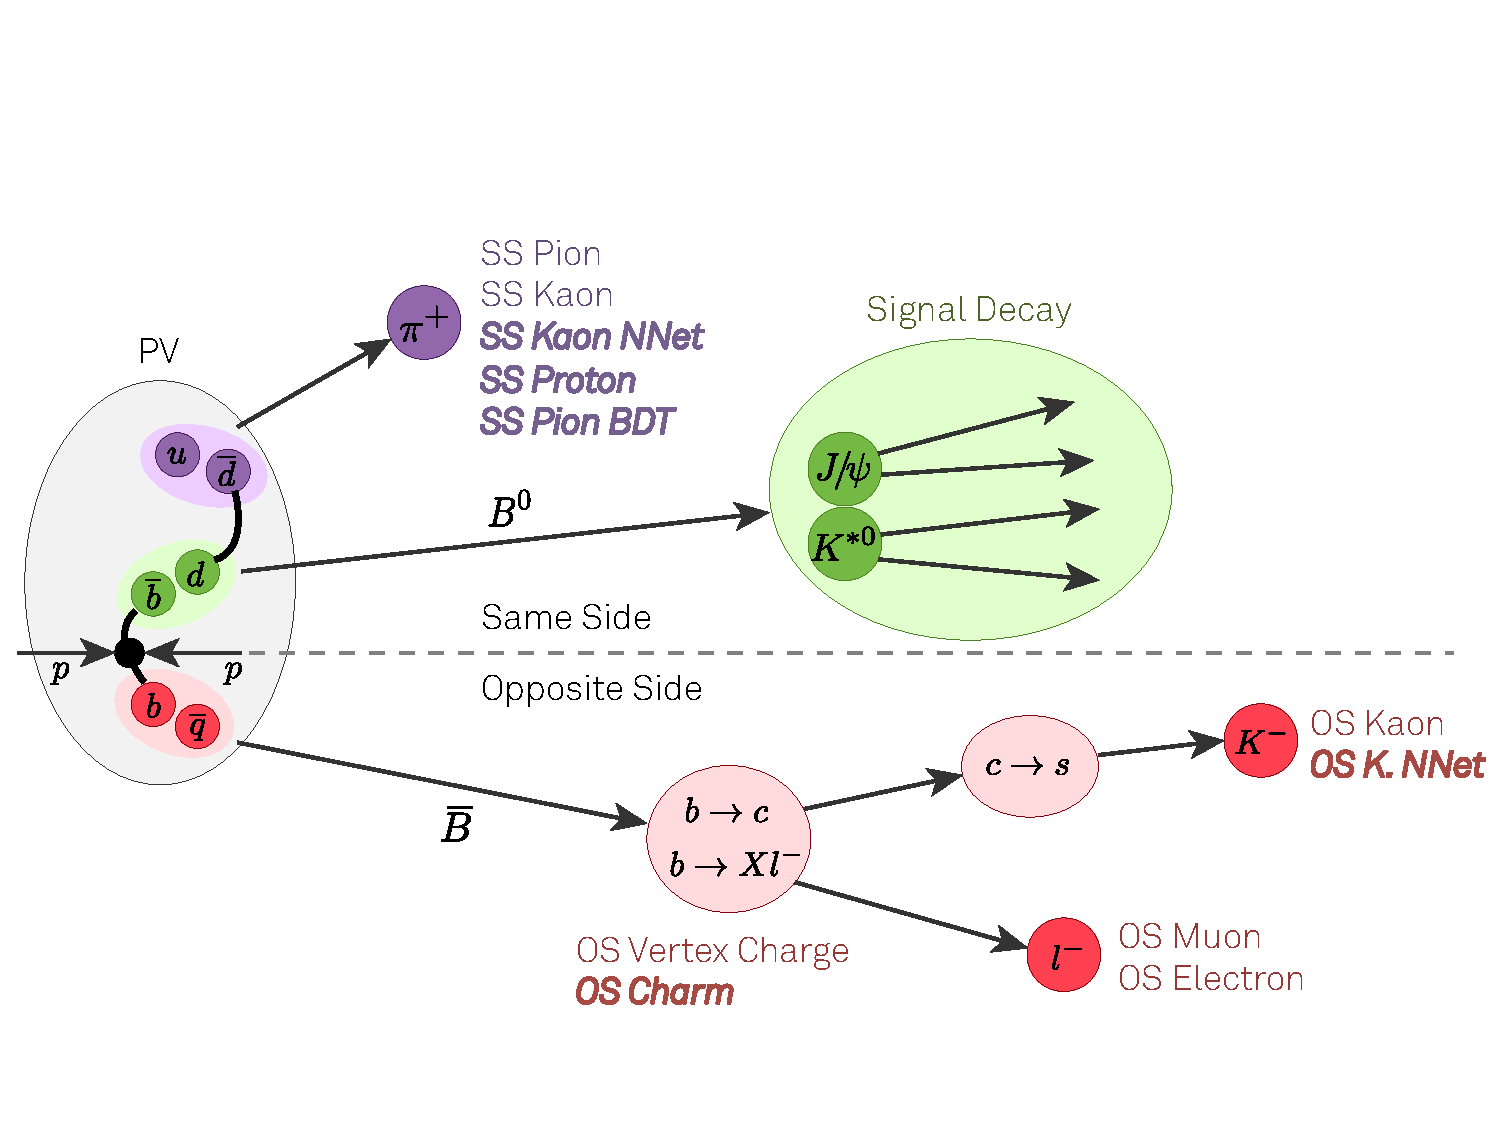
\includegraphics[width=\textwidth]{images/FlavourTaggingScheme.pdf}

      \tiny \url{https://twiki.cern.ch/twiki/bin/view/LHCb/FlavourTaggingConferencePlots}
    \end{column}
    \begin{column}{0.4\textwidth}
      \begin{itemize}
        \item $pp$-collisions produce many particles
        \item gluon-fusion may lead to a $b\bar{b}$-pair
        \item hadronisation $\rightarrow$ $B$ meson and fragmentation particles
        \item Lorentz boosted signal $B$ $\rightarrow$ distinguish secondary from primary vertex
        \item for $B^0_d$ vs $B^0_s$ only same side (SS) relevant
        \item here: exclude the signal decay
      \end{itemize}
    \end{column}
  \end{columns}
\end{frame}

\begin{frame}{The LHCb detector}
  \centering
  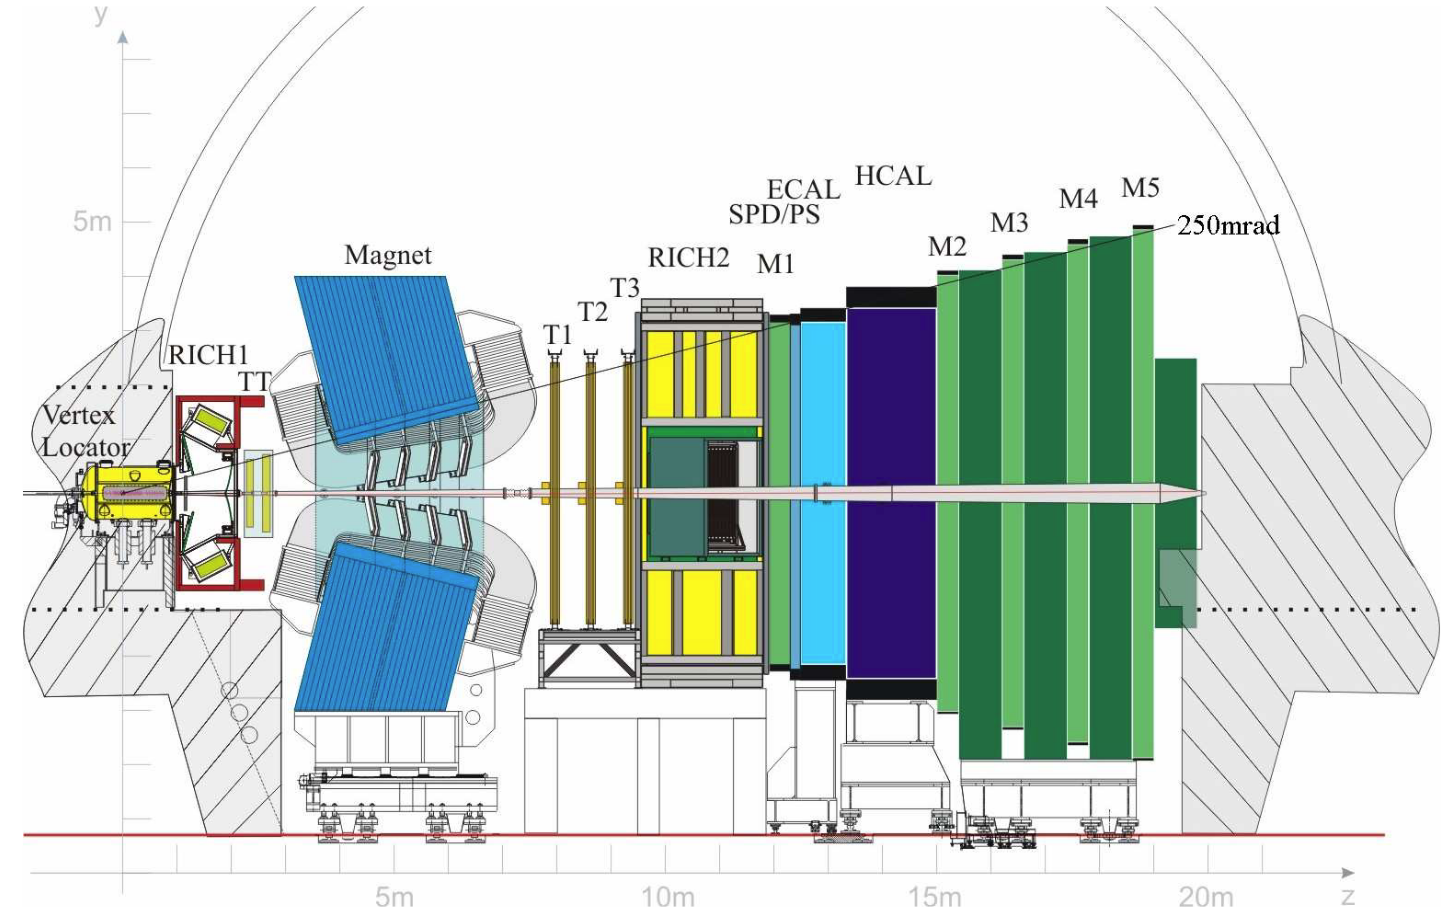
\includegraphics[height=0.9\textheight]{images/lhcb_detector.png}

  \tiny \url{https://iopscience.iop.org/article/10.1088/1748-0221/3/08/S08005}
\end{frame}

\section*{Development of a B meson classifier}

\begin{frame}{Development of a $B$ meson classifier}
  \centering
  \begin{columns}
    \begin{column}{0.6\textwidth}
      \textbf{Strategy:}
      \begin{itemize}
        \item same side track identification using a BDT
        \item $B$ meson classification using a DeepSet
        \item test on real LHCb data
      \end{itemize}

      \pause
      \textbf{Training dataset:}
      \begin{itemize}
        \item training with LHCb simulation
        \item combined dataset:
        \begin{itemize}
          \item $B^0_d \rightarrow J/\psi K^*$
          \item $B^0_s \rightarrow D_s^+ \pi^-$
        \end{itemize}
        \item found differences by year and simulation version \\$\rightarrow$ chose 2016 and same simulation version
        \item dataset contains 0.4 million events and 18 million tracks
      \end{itemize}
    \end{column}
  \end{columns}
\end{frame}

\section*{SS track identification using a BDT}

\begin{frame}{Boosted Decision Tree (BDT)}
  \begin{columns}
    \begin{column}{0.5\textwidth}
      \centering
      \textbf{Simple Decision Tree:}
      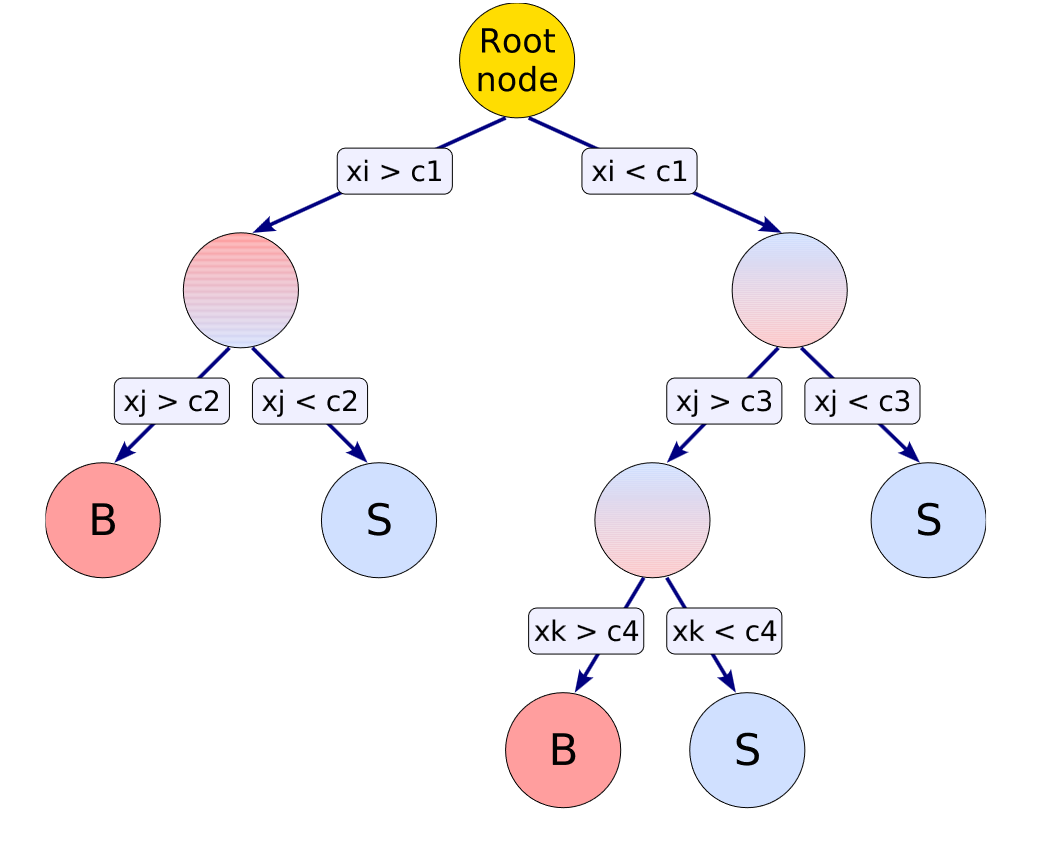
\includegraphics[width=\textwidth]{images/decision_tree.png}

      \tiny \url{https://arxiv.org/abs/physics/0703039}
    \end{column}
    \pause
    \begin{column}{0.5\textwidth}
      \textbf{Boosted Decision Tree:}
      \begin{itemize}
        \item ensemble of multiple small Decision Trees
        \item weighted sum transformed with logistic function \\$\rightarrow$ estimated class probabilities
        \item iterative training through gradient boosting \\$\rightarrow$ minimum of a loss function
      \end{itemize}
    \end{column}
  \end{columns}
\end{frame}

\begin{frame}{SS track identification: Feature Selection}
  \begin{columns}
    \begin{column}{0.3\textwidth}
      \centering
      \begin{tabular}{c c}
        \toprule
        \multicolumn{2}{c}{track features} \\
        \midrule
        $p_\text{T}$        & $\text{IP}_\text{SV}$ \\ 
        $p_\text{proj}$     & $\chi^2(\text{IP}_\text{SV})$ \\ 
        $\Delta p_\text{T}$ & $\sigma(\text{IP}_\text{pileup vtx})$ \\ 
        $\Delta z$          & $\text{IP}_\text{best PV}$ \\    
        $\Delta \eta$       & $\chi^2(\text{IP}_\text{best PV})$ \\ 
        $\cos(\Delta \phi)$ & $\text{IP}_\text{min}$ \\ 
        $\text{Prob}_\text{ghost}$ & same PV \\
        $\chi^2(\text{vtx})$     & cone isolation \\
        SumBDT              & $N_\text{non iso}$ \\ 
        MinBDT              & $\sum p_\text{in cone}$ \\ 
        SumMinBDT           &  \\
        \bottomrule
      \end{tabular}
    \end{column}
    \begin{column}{0.7\textwidth}
      \centering
      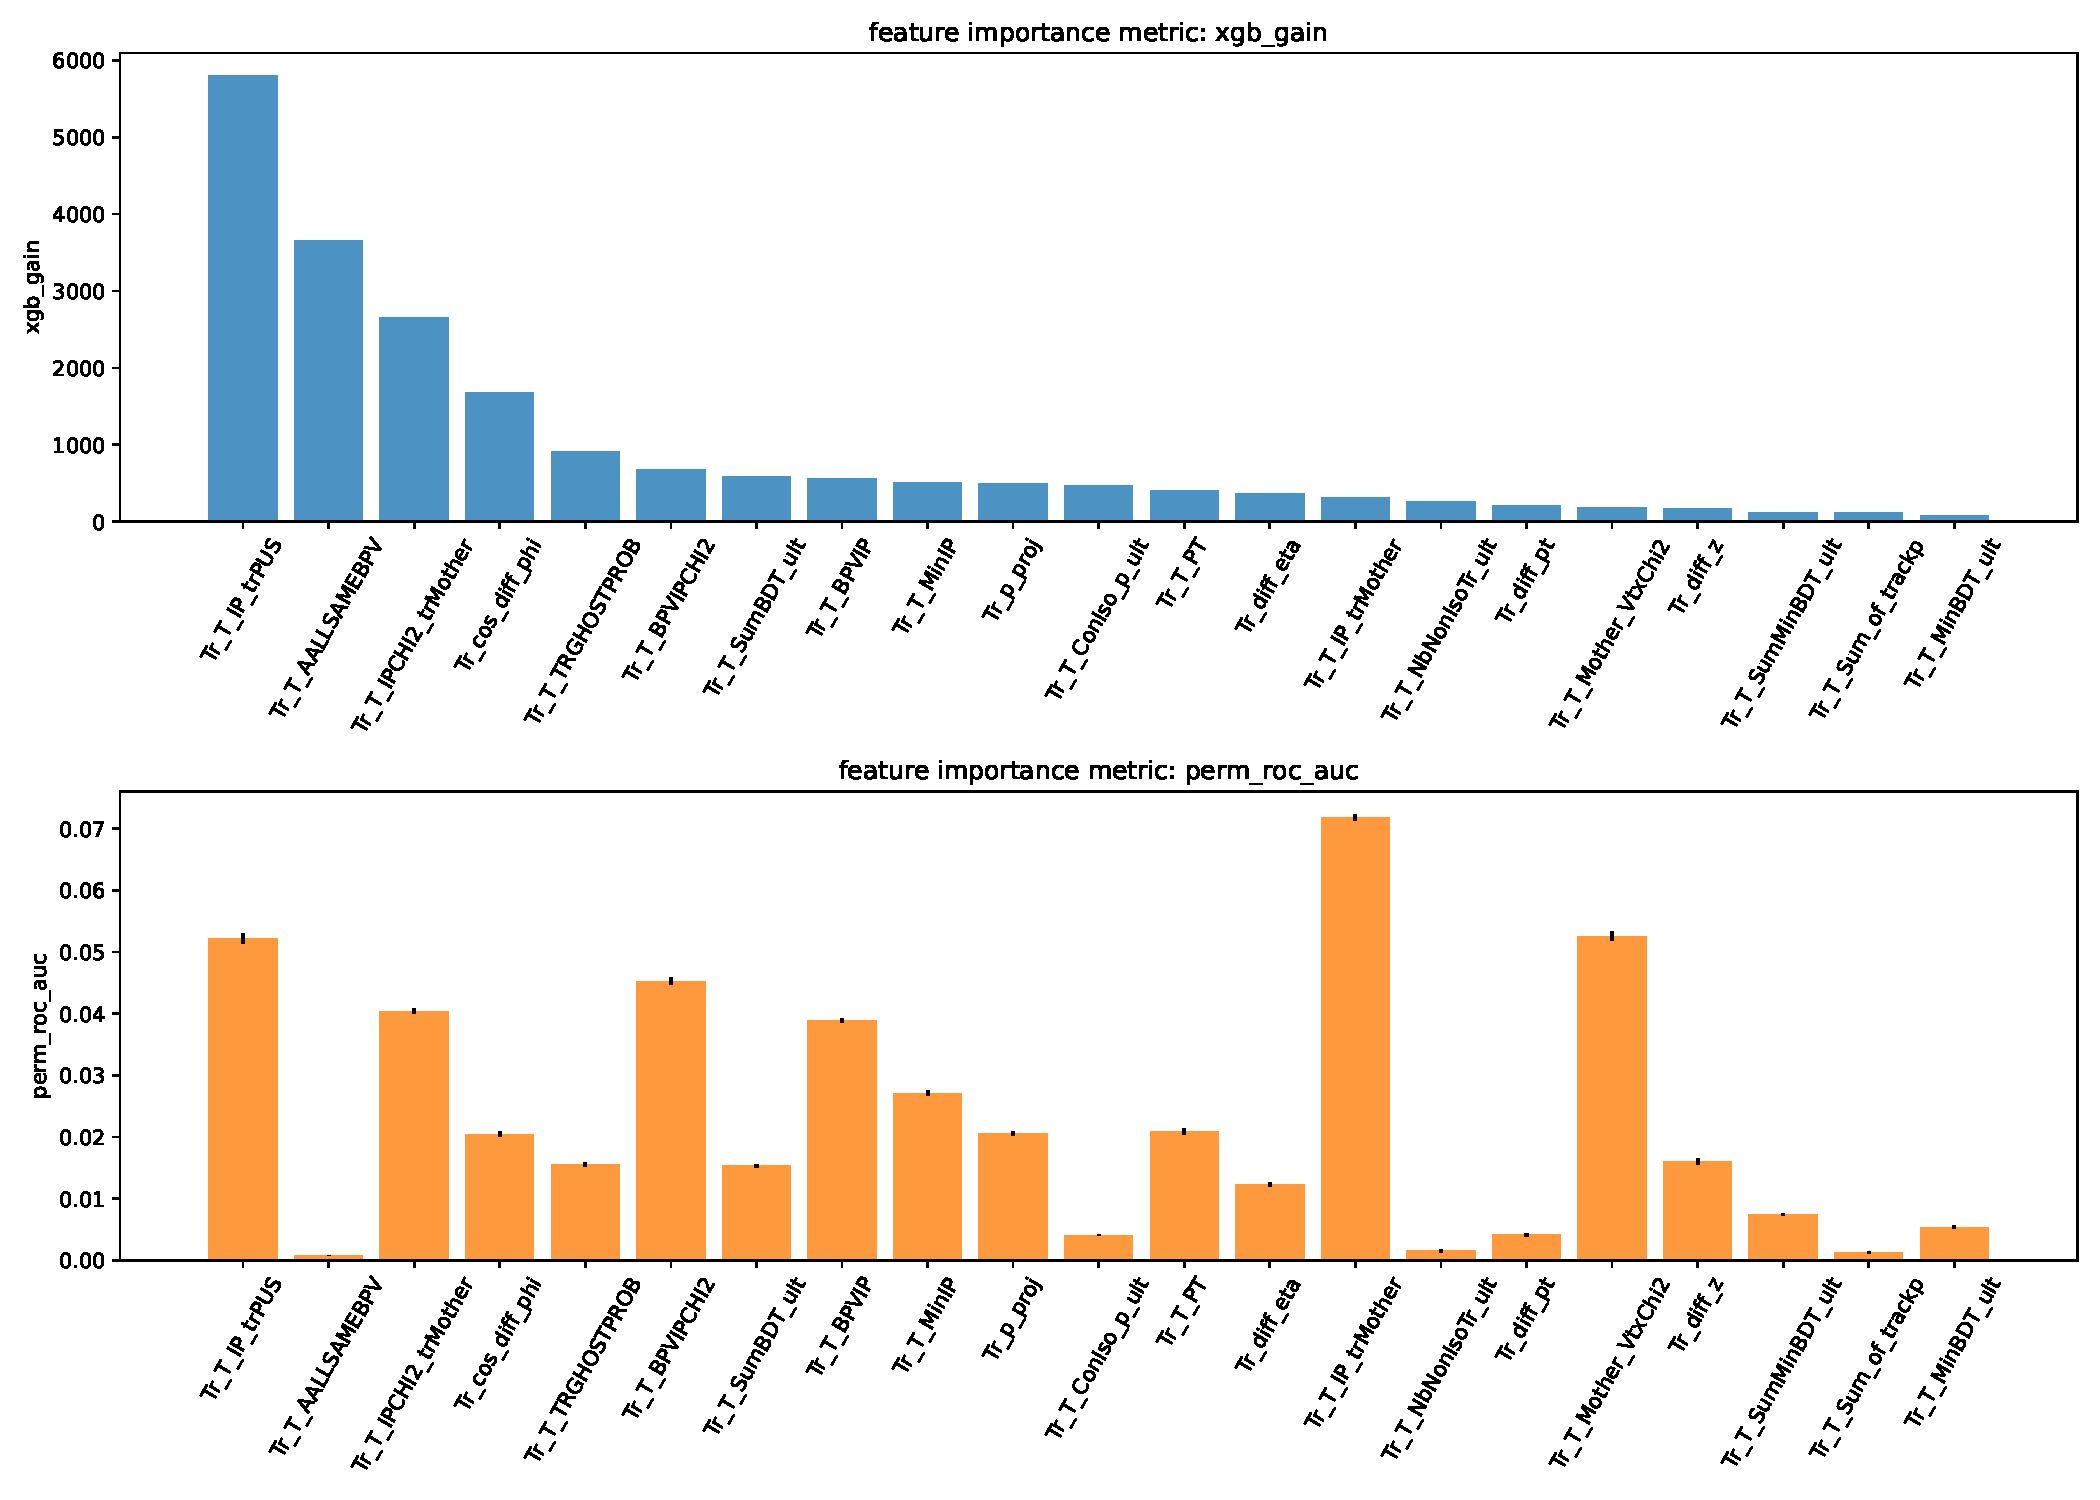
\includegraphics[width=\textwidth]{images/SS_feature_importances.pdf}
    \end{column}
  \end{columns}
\end{frame}

\begin{frame}{SS track identification: BDT training and results}
  \begin{columns}
    \begin{column}{0.5\textwidth}
      \centering
      \only<1>{%
        \textbf{Error rate during training}
        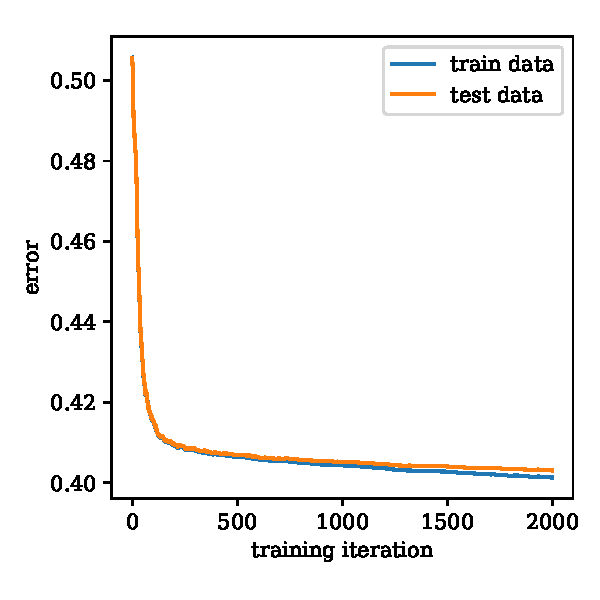
\includegraphics[width=0.85\textwidth]{images/SS_history_error.pdf}
      }
      \only<2-3>{%
        \textbf{Distribution of $\text{Prob}_\text{SS}$}
        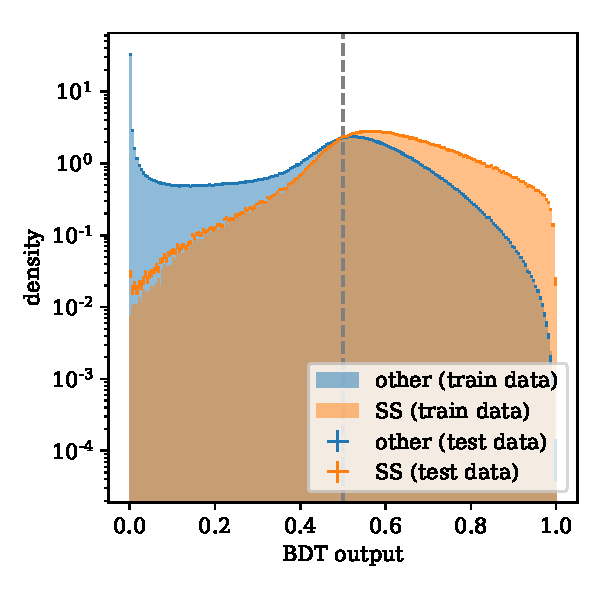
\includegraphics[width=0.85\textwidth]{images/SS_output.pdf}
      }
    \end{column}
    \begin{column}{0.5\textwidth}
      \only<1-2>{%
        \begin{itemize}
          \item 60\% training data, 40\% test data
          \item 2000 decision trees with maximum tree depth of 4
          \item loss: logistic regression for binary classification
          \item output: $\text{Prob}_\text{SS} \in [0,1]$
        \end{itemize}
      }
      \only<3>{%
        \centering
        \textbf{ROC curve of the BDT predictions}
        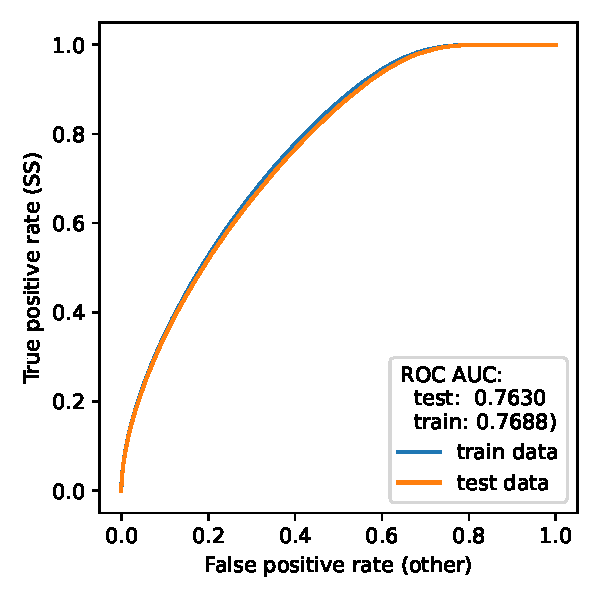
\includegraphics[width=0.85\textwidth]{images/SS_ROC.pdf}
      }
    \end{column}
  \end{columns}
\end{frame}

\section*{B meson classification using a DeepSet}

\begin{frame}{Neural Network (NN)}
  \begin{columns}
    \begin{column}{0.5\textwidth}
      \centering
      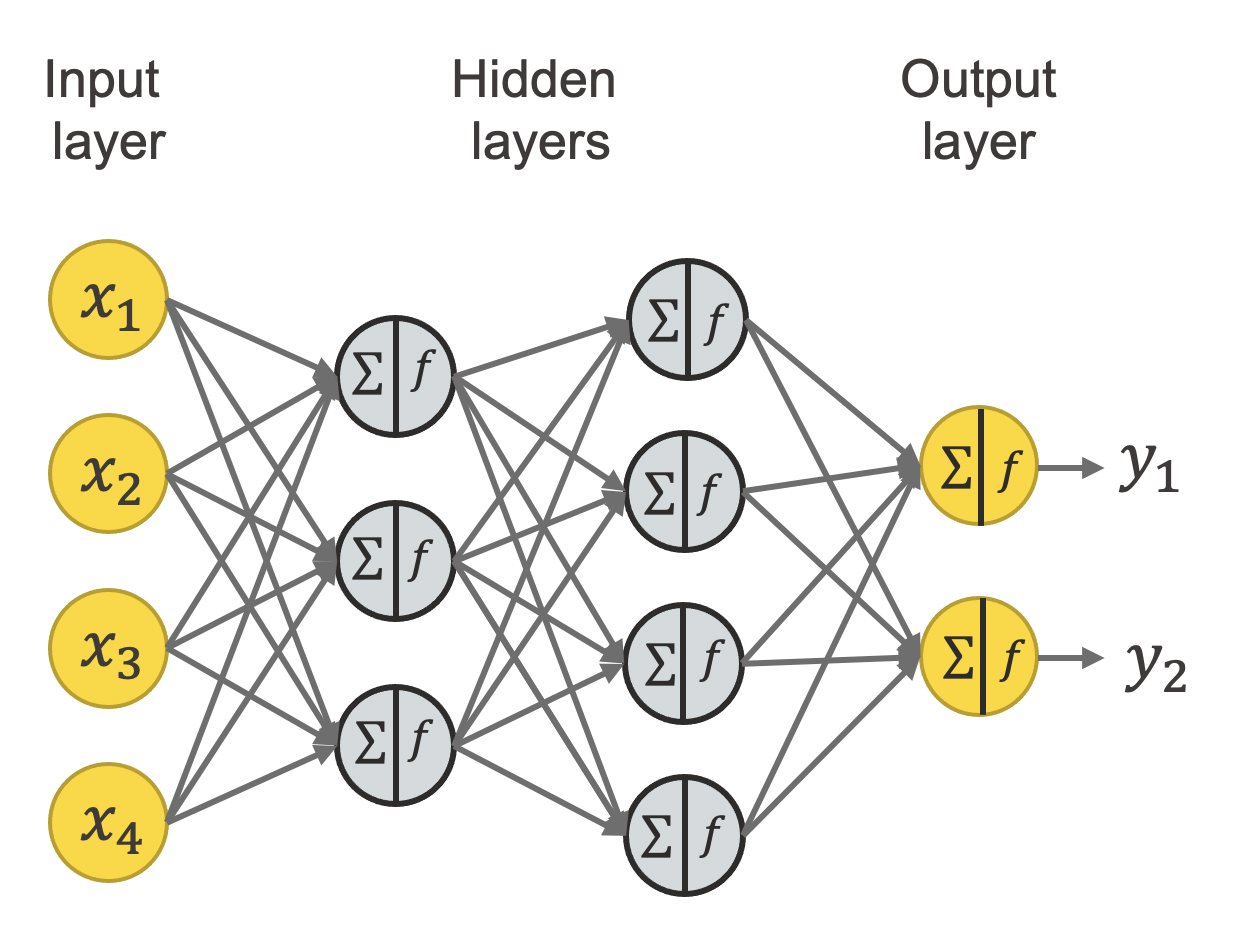
\includegraphics[width=0.85\textwidth]{images/NN_schematic.png}

      \tiny \url{https://www.knime.com/blog/a-friendly-introduction-to-deep-neural-networks}
    \end{column}
    \begin{column}{0.5\textwidth}
      \begin{itemize}
        \item non-linear transformation $\vec{x} \rightarrow \vec{y}$
        \item multiple steps called layers of activation \\$\rightarrow$ $\vec{a}^{(n)} = f^{(n)}\left( W^{(n)} \cdot \vec{a}^{(n-1)} + \vec{b}^{n} \right)$
        \item activation functions used here:
        \begin{itemize}
          \item $f_\text{ReLU}(z) = \max (0, z)$
          \item $f_\text{Sigmoid}(z) = \frac{1}{1+e^{-z}}$
        \end{itemize}
        \item iterative training through backpropagation (gradient descent)
      \end{itemize}
    \end{column}
  \end{columns}
\end{frame}

\begin{frame}{DeepSet}
  \begin{columns}
    \begin{column}{0.5\textwidth}
      \begin{itemize}
        \item extension of NNs to allow inputs of sets of vectors \\
        $\rightarrow$ variable input length \\
        $\rightarrow$ permutation invariant
        \item $\displaystyle f(X) = \rho \left( \sum_{x_i \in \text{ \normalsize{$X$}}} \phi(x_i) \right)$
      \end{itemize}

      \medskip
      \centering
      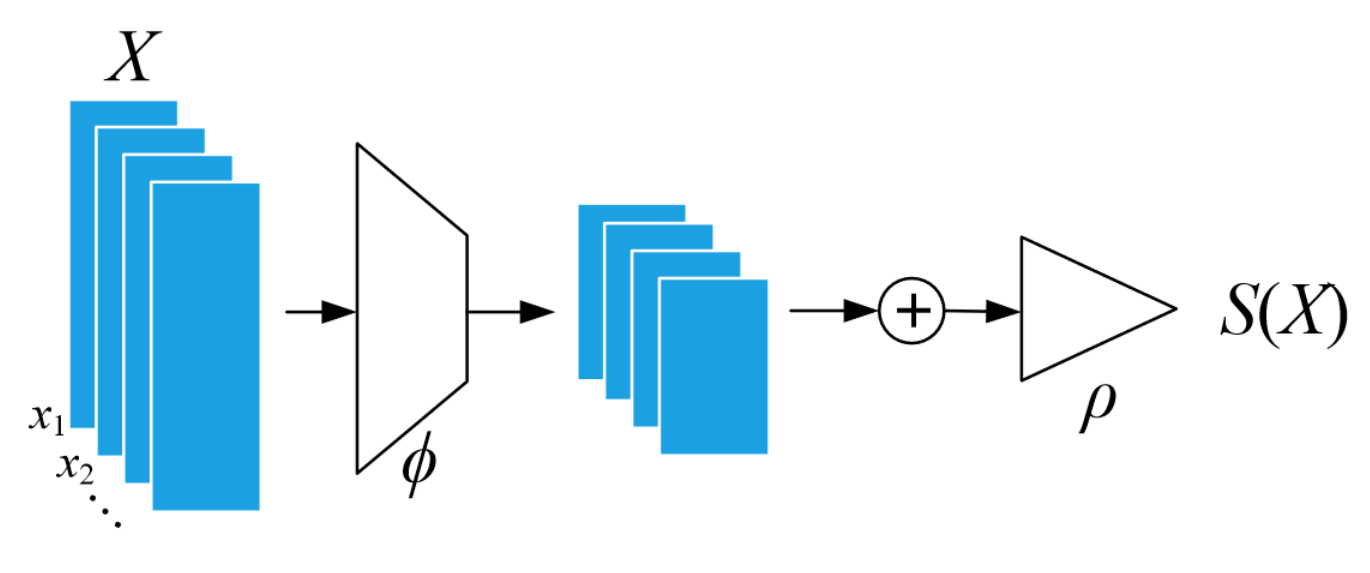
\includegraphics[width=0.9\textwidth]{images/DeepSet_schematic.png}

      \tiny \url{https://arxiv.org/abs/1703.06114}
    \end{column}
    \begin{column}{0.5\textwidth}
      \pause
      \textbf{DeepSet for B meson classification:}
      \begin{itemize}
        \item one set $X$ per event
        \item one vector $x_i$ per track
        \item $\phi$-network layer sizes: 23, 64, 128, 64
        \item $\rho$-network layer sizes: 64, 128, 64, 1
        \item $f_\text{ReLU}$ for hidden layers  
        \item $f_\text{Sigmoid}$ for the output layer
        \item output: $\text{Prob}_{B_s} \in [0,1]$
      \end{itemize}
    \end{column}
  \end{columns}
\end{frame}

\begin{frame}{B meson classification: Feature Selection}
  \begin{columns}
    \begin{column}{0.25\textwidth}
      \centering
      \begin{tabular}{c c}
        \toprule
        \multicolumn{2}{c}{track features} \\
        \midrule
        $p$                 & $\text{\textbf{Prob}}_\text{\textbf{SS}}$ \\ %"Tr_T_P","Tr_ProbSS"
        $p_\text{T}$        & $\text{Prob}_e$ \\ %"Tr_T_PT", "Tr_T_PROBNNe"
        $p_\text{proj}$     & $\text{Prob}_\text{ghost}$ \\ %"Tr_p_proj","Tr_T_PROBNNghost"
        $\Delta p$          & $\text{Prob}_K$ \\ %"Tr_diff_p", "Tr_T_PROBNNk"
        $\Delta p_\text{T}$ & $\text{Prob}_\mu$ \\ %"Tr_diff_pt","Tr_T_PROBNNmu"
        $\Delta z$          & $\text{Prob}_p$ \\ %"Tr_diff_z", "Tr_T_PROBNNp"
        $\cos(\Delta \phi)$ & $\text{Prob}_\pi$ \\ %"Tr_cos_diff_phi", "Tr_T_PROBNNpi"
        $\Delta \eta$       & $\sigma(\text{IP}_\text{pileup vtx})$ \\ %"Tr_diff_eta", "Tr_T_IP_trPUS"
        $\text{IP}_\text{SV}$        & $Q_\text{VELO}$ \\ %"Tr_T_IP_trMother",  "Tr_T_VeloCharge"
        $\chi^2(\text{IP}_\text{SV})$    & SumBDT \\ %"Tr_T_IPCHI2_trMother", "Tr_T_SumBDT_ult"
        $\text{IP}_\text{min}$               & MinBDT \\ %"Tr_T_MinIP", "Tr_T_MinBDT_ult"
        $\chi^2(\text{IP}_\text{min})$           & \\ %"Tr_T_MinIPChi2"
        \bottomrule
    \end{tabular}
    \end{column}
    \begin{column}{0.75\textwidth}
      \centering
      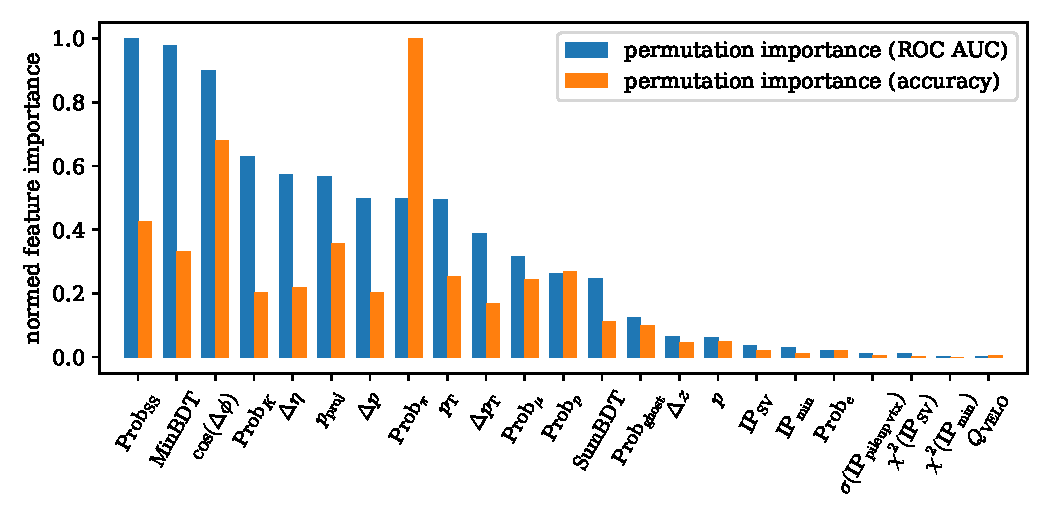
\includegraphics[width=\textwidth]{images/B_feature_importances.pdf}
    \end{column}
  \end{columns}
\end{frame}

\begin{frame}{B meson classification: DeepSet training and results}
  
  \begin{columns}
    \begin{column}{0.5\textwidth}
      \centering
      \only<1>{%
        \textbf{Error rate during training}
        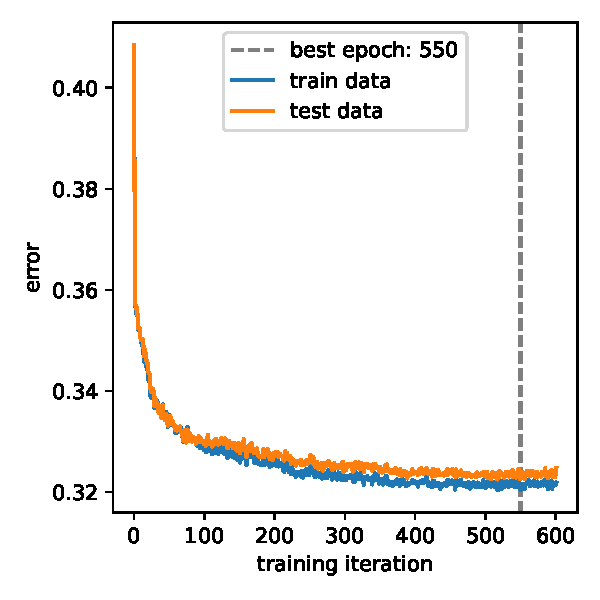
\includegraphics[width=0.85\textwidth]{images/B_history_error.pdf}
      }
      \only<2-3>{%
        \textbf{Distribution of $\text{Prob}_{B_s}$}
        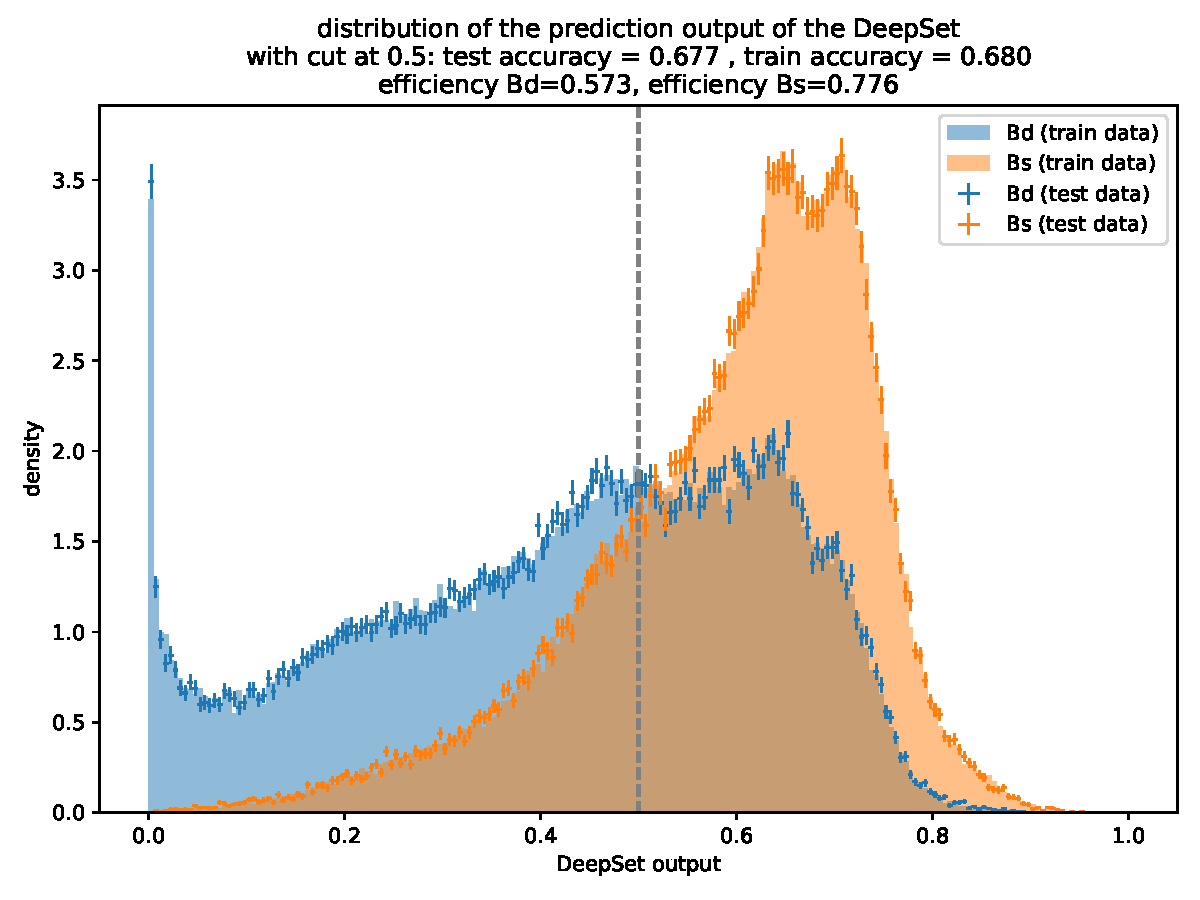
\includegraphics[width=0.85\textwidth]{images/B_output.pdf}
      }
    \end{column}
    \begin{column}{0.5\textwidth}
      \only<1-2>{%
        \begin{itemize}
          \item 60\% training data, 40\% test data (standard scaled)
          \item regularisation: 
          \begin{itemize}
            \item early stopping after 50 iterations
            \item Dropout of 50\%
          \end{itemize}
          \item loss: binary cross entropy
          \item optimizer: Adam
          \item output: $\text{Prob}_{B_s} \in [0,1]$
        \end{itemize}
      }
      \only<3>{%
        \centering
        \textbf{ROC curve of the DeepSet predictions}
        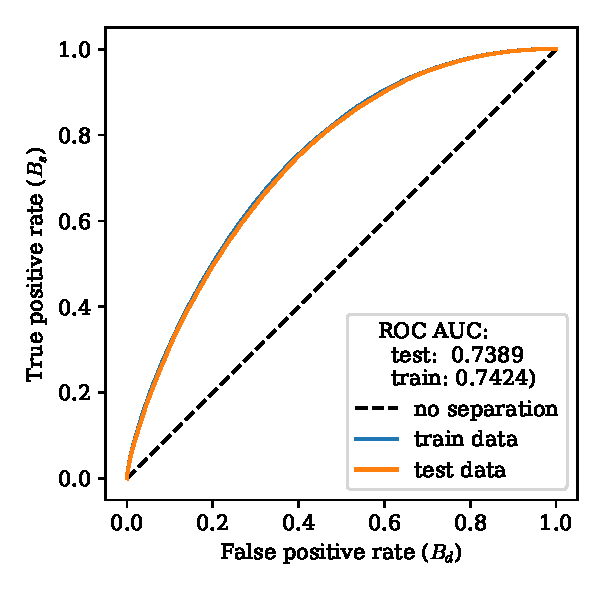
\includegraphics[width=0.85\textwidth]{images/B_ROC.pdf}
      }
    \end{column}
  \end{columns}
\end{frame}

\section*{Testing on LHCb data}

\begin{frame}{Testing on LHCb data: Overview}
  \begin{columns}[t]
    \begin{column}{0.5\textwidth}
      \begin{itemize}
        \item run 2 LHCb data selected for $B^0_d \, \text{or} \, B^0_s \rightarrow J/\psi K^0_S$
        \item based on an existing analysis
        \only<2>{%
          \item visible $B^0_s$ peak after background reduction:
          \begin{itemize}
            \item trained BDT with 13 features on \\
            $B^0_d \rightarrow J/\psi K^0_S$ simulation as signal and \\
            mass sideband ($\geq \qty{5450}{\MeV}$) as combinatorial background
            \item manual cuts for $\Lambda^0$ and $K^*$ background\\
            that got misidentified as $K^0_S$
          \end{itemize}
        }
        \only<3->{%
          \item visible $B^0_s$ peak after background reduction
          \item testing strategy:
          \begin{itemize}
            \item apply the developed algorithm \\$\rightarrow$ $\text{Prob}_{B_s}$ for every event
            \item estimate counts of $B^0_d$ and $B^0_s$ events by\\
            fitting the mass distribution and \\
            integrating the $B^0_d$ and $B^0_s$ components
            \item scan through the $\text{Prob}_{B_s}$ distribution
          \end{itemize}
        }
      \end{itemize}
    \end{column}
    \begin{column}{0.5\textwidth}
      \centering
      \only<1-3>{\visible<2-3>{%
        \textbf{Signal B mass after background reduction\\
        (peaks at $M_{B_d} = \qty{5280}{\MeV}$ and $M_{B_s} = \qty{5367}{\MeV}$)}
        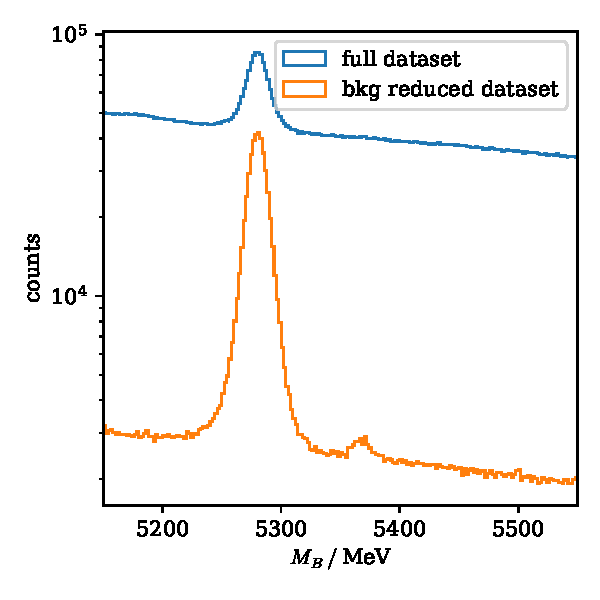
\includegraphics[width=0.85\textwidth]{images/BKG_reduced.pdf}
      }}
      \only<4>{%
        \textbf{Example fit of the mass distribution}
        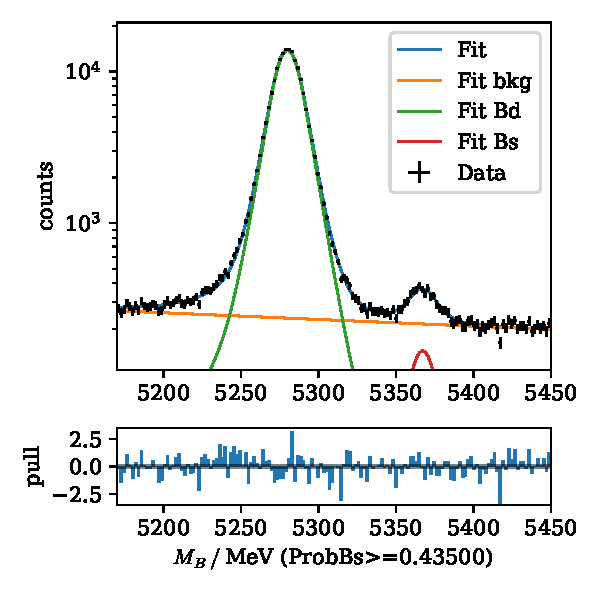
\includegraphics[width=0.85\textwidth]{images/fit_example_new.pdf}
      }
    \end{column}
  \end{columns}  
\end{frame}

\begin{frame}{Testing on LHCb data: Results (ratio $n_{B_s}/n_{B_d}$ by $\text{Prob}_{B_s}$ cut value)}
  \centering
  \begin{columns}
    \begin{column}{0.5\textwidth}
      \centering
      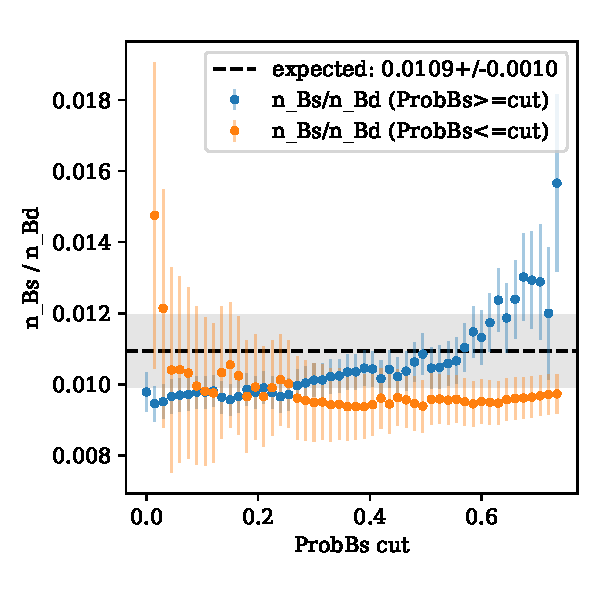
\includegraphics[width=\textwidth]{images/ratio_data.pdf}
    \end{column}
  \end{columns}
\end{frame}

\begin{frame}{Testing on LHCb data: Animation of $n_{B_s}/n_{B_d}$ and the corresponding fits}
  \animategraphics[loop,controls,palindrome,width=\linewidth]{5}{images/ratio_animation/frame_}{0}{48}
\end{frame}

\begin{frame}{Testing on LHCb data: Results (ratio $n_{B_s}/n_{B_d}$ by $\text{Prob}_{B_s}$ cut value)}
  \begin{columns}
    \begin{column}{0.45\textwidth}
      \centering
      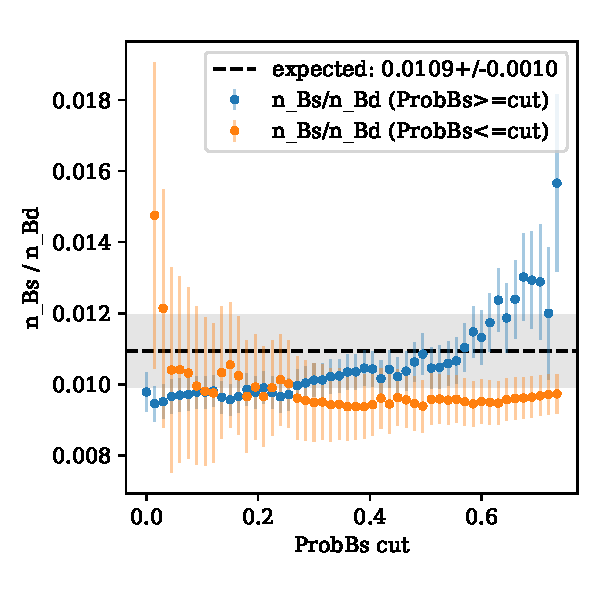
\includegraphics[width=\textwidth]{images/ratio_data.pdf}
    \end{column}
    \begin{column}{0.55\textwidth}
      \begin{itemize}
        \item without separation: constant ratio $n_{B_s}/n_{B_d}$
        \item expected value (with perfect selection efficiencies):
        \begin{equation*}
          \frac{\text{BR}(B_s \rightarrow J/\psi \, K^0_\text{S})}{\text{BR}(B_d \rightarrow J/\psi \, K^0_\text{S})} \cdot f_s/f_d(\qty{13}{\TeV}) = \num{0.0109\pm0.0010}
        \end{equation*}
        \pause
        \item $\text{Prob}_{B_s} \leq x$: mostly constant, no clear $B^0_s$ peak for low $x$
        \pause
        \item $\text{Prob}_{B_s} \geq x$: starts constant, then increases
        \pause 
        \item clearly achieved some separation between $B^0_d$ and $B^0_s$
        \item comparison to the simulation?
      \end{itemize}
    \end{column}
  \end{columns}
\end{frame}

\begin{frame}{Testing on LHCb data: Results (ratio $n_{B_s}/n_{B_d}$ by $\text{Prob}_{B_s}$ cut value)}
  \begin{columns}
    \begin{column}{0.5\textwidth}
      \centering
      \textbf{Achieved separation on data}
      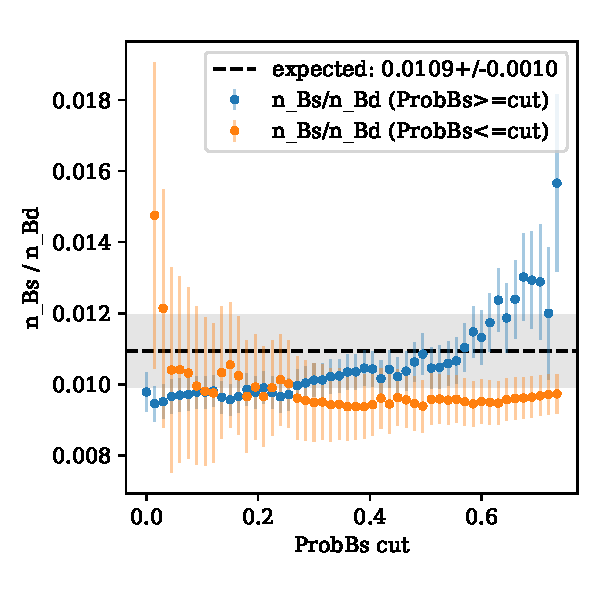
\includegraphics[width=0.9\textwidth]{images/ratio_data.pdf}
    \end{column}
    \begin{column}{0.5\textwidth}
      \centering
      \textbf{Achieved separation on simulation}
      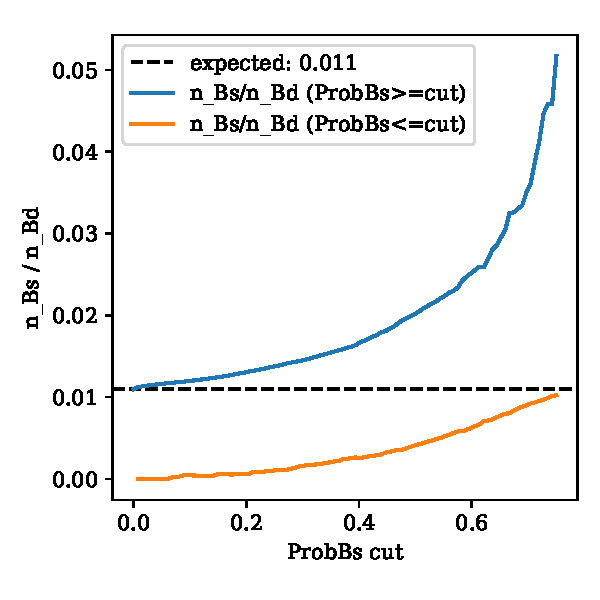
\includegraphics[width=0.9\textwidth]{images/ratio_mc.pdf}
    \end{column}
  \end{columns}
\end{frame}

\section*{Conclusion and outlook}

\begin{frame}{Conclusion and outlook}
  \textbf{Results:}
  \begin{itemize}
    \item BDT can identify SS tracks (ROC AUC: 0.76) and helps the DeepSet (feature importances)
    \item DeepSet achieves clear separation of $B^0_d$ and $B^0_s$ events on the simulated test sample (ROC AUC: 0.74)
    \item separation on LHCb data cannot be quantified
    \begin{itemize}
      \item some level of separation seen in $n_{B_s}/n_{B_d}$
      \item no sign of separation in ROC curve
    \end{itemize}
    \item reasons for performance loss unknown (selection differences? mismodeled simulation?)
  \end{itemize}
  
  \pause
  \medskip
  \textbf{Outlook and suggestions:}
  \begin{itemize}
    \item indications that a similar approach could succeed
    \item compare simulation kinematics with real world kinematics
    \item ensure that kinematic differences originate from the mass difference
    \item potentially equalize the kinematics by reweighting the training data
    \item if successful, extension to include charged $B$ mesons possible
  \end{itemize}
\end{frame}

\appendix

\begin{frame}[plain]
  \centering
  \begin{beamercolorbox}[center, wd=\textwidth]{title}
    \textcolor{tugreen}{\rule{\textwidth}{1pt}}\\[0.5\baselineskip]%
    \usebeamerfont{title}Thank you for your attention!
    \\[0.5\baselineskip]%
    \usebeamerfont{subtitle}Here is some art I found in the data (2D histograms):\newline%
    \textcolor{tugreen}{\rule{\textwidth}{1pt}}%
  \end{beamercolorbox}%
  \begin{columns}
    \begin{column}{0.5\textwidth}
      \centering
      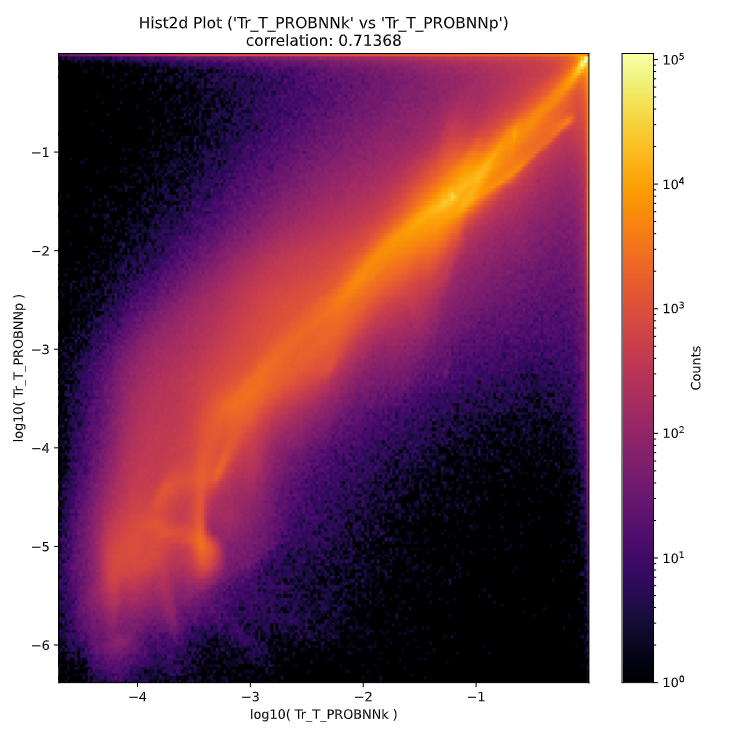
\includegraphics[width=1.1\textwidth]{images/backup/art1.png}
    \end{column}
    \begin{column}{0.5\textwidth}
      \centering
      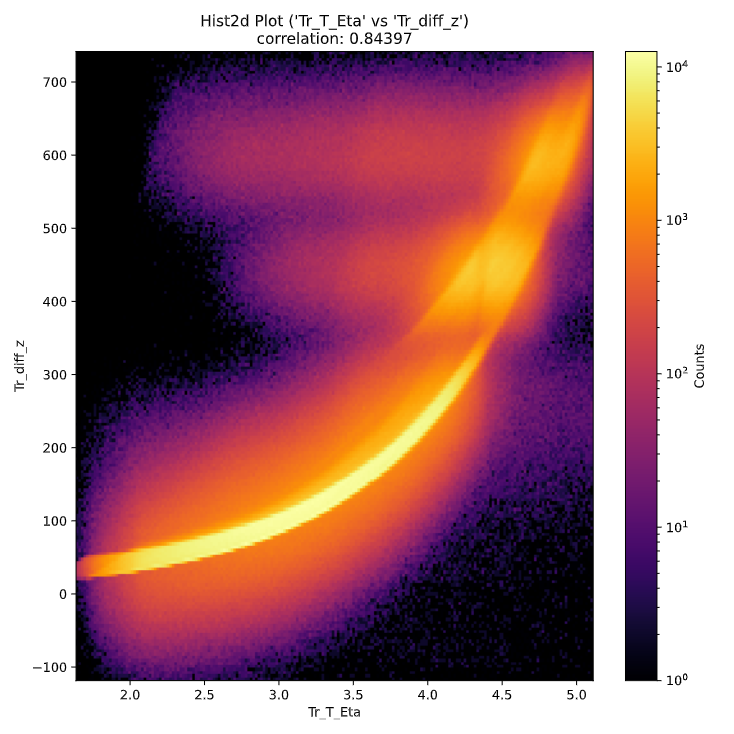
\includegraphics[width=1.1\textwidth]{images/backup/art2.png}
    \end{column}
  \end{columns}
\end{frame}


%%%%%%%%%%%%%%%%%%%%%%%%%%%%%%%%%%%%%%%%%%%%%%%%%%%%%%%%

\begin{frame}[plain]
  \centering
  \begin{beamercolorbox}[center, wd=\textwidth]{title}
    \textcolor{tugreen}{\rule{\textwidth}{1pt}}\\[0.5\baselineskip]%
    \usebeamerfont{title}Backup
    \textcolor{tugreen}{\rule{\textwidth}{1pt}}%
  \end{beamercolorbox}%
\end{frame}

\begin{frame}{Correlation Matrix}
  \centering
  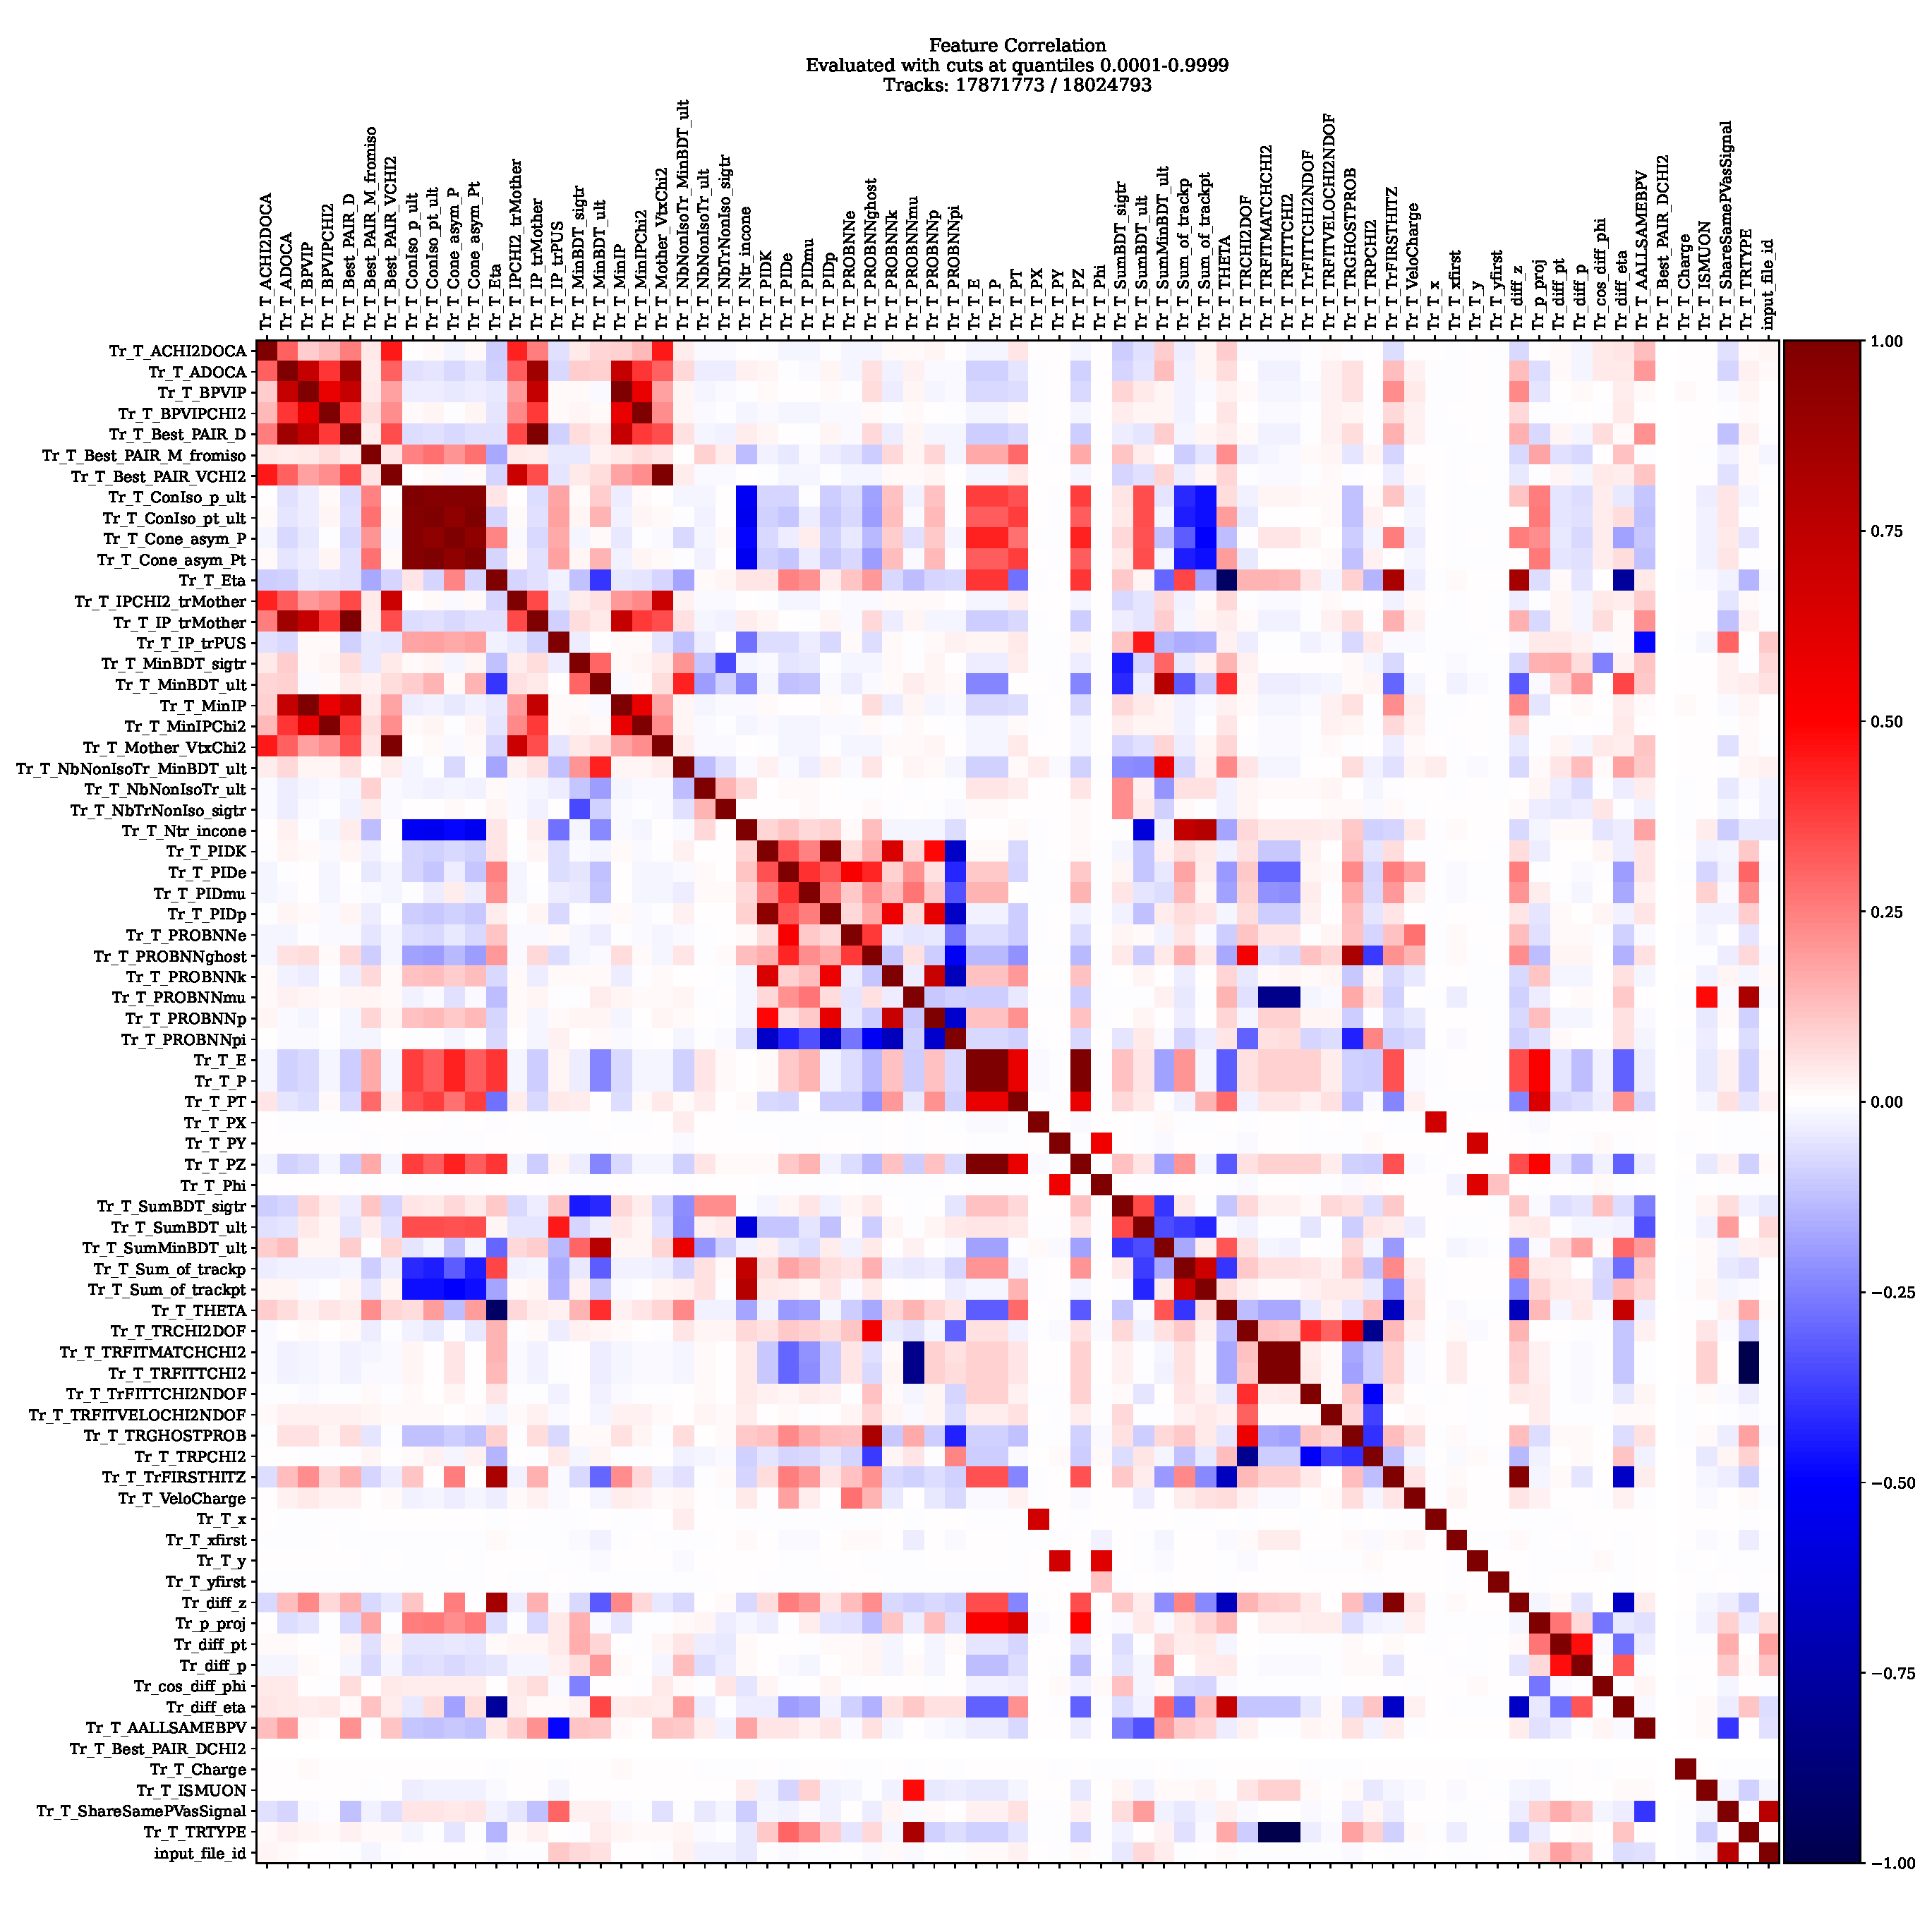
\includegraphics[height=0.9\textheight]{images/backup/correlation_matrix.pdf}
\end{frame}

\begin{frame}{Background BDT}
  \begin{columns}
    \begin{column}{0.33\textwidth}
      \centering
      \begin{tabular}{c c}
        \toprule
        \multicolumn{2}{c}{signal features} \\
        \midrule
        IP$(B^0)$                   & $p_\text{T}(\pi^+)$ \\% "B_IP_OWNPV","piplus_PT"
        IP$(J/\psi)$                & $p_\text{T}(\pi^-)$ \\% "Jpsi_IP_OWNPV","piminus_PT"
        IP$(K^0_\text{S})$          & $p_\text{T}(K^0_\text{S})$ \\% "KS0_IP_OWNPV","KS0_PT"
        IP$(\mu^+)$                 & $\eta(B^0)$ \\% "muplus_IP_OWNPV","B_LOKI_ETA"
        IP$(\mu^-)$                 & $\eta(K^0_\text{S})$ \\% "muminus_IP_OWNPV","KS0_LOKI_ETA"
        FD$(K^0_\text{S})$    & $p_z(K^0_\text{S})$ \\% "KS0_FD_OWNPV","KS0_PZ"
        $\chi^2(\text{fit})$  & \\% "B_LOKI_DTF_CHI2NDOF",
        \bottomrule
    \end{tabular}
    \end{column}
    \begin{column}{0.33\textwidth}
      \centering
      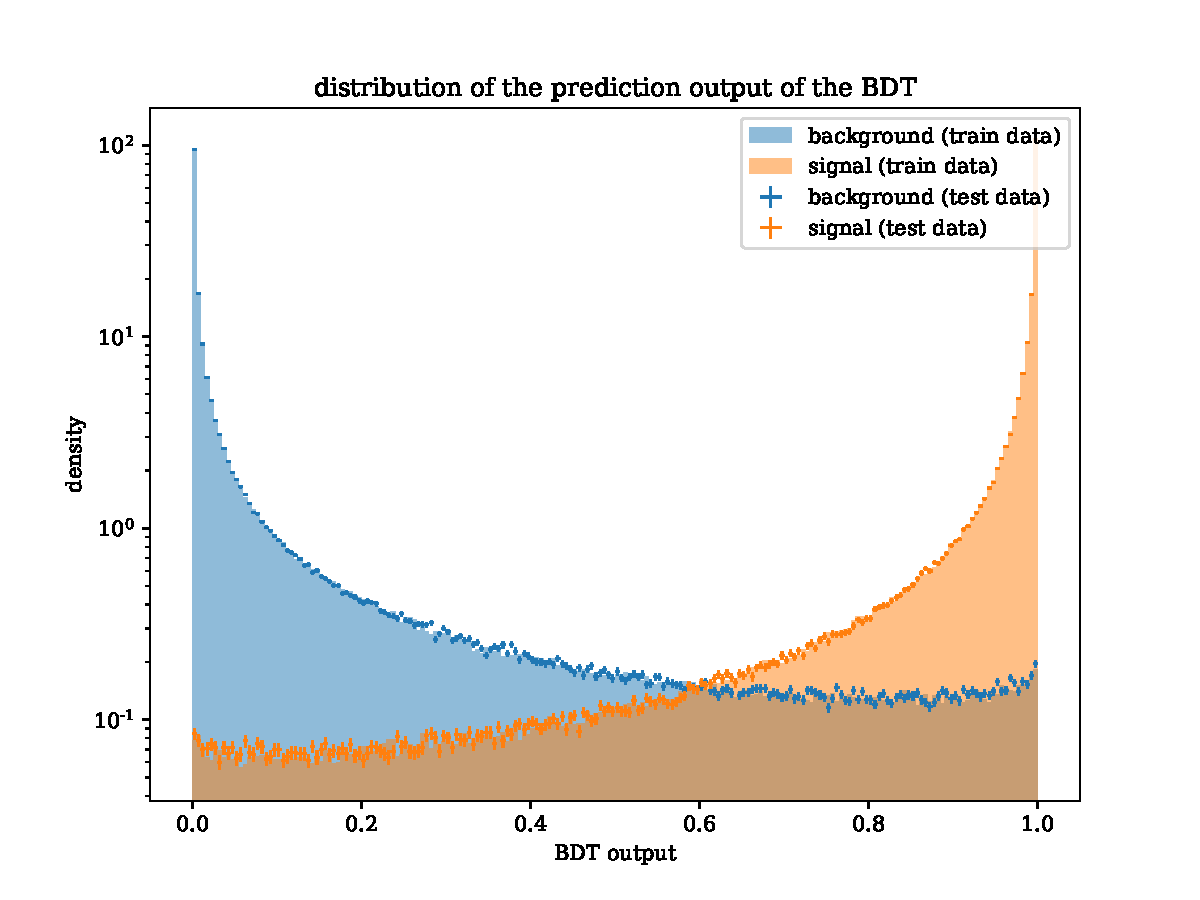
\includegraphics[width=\textwidth]{images/backup/bkg_output.pdf}
    \end{column}
    \begin{column}{0.33\textwidth}
      \centering
      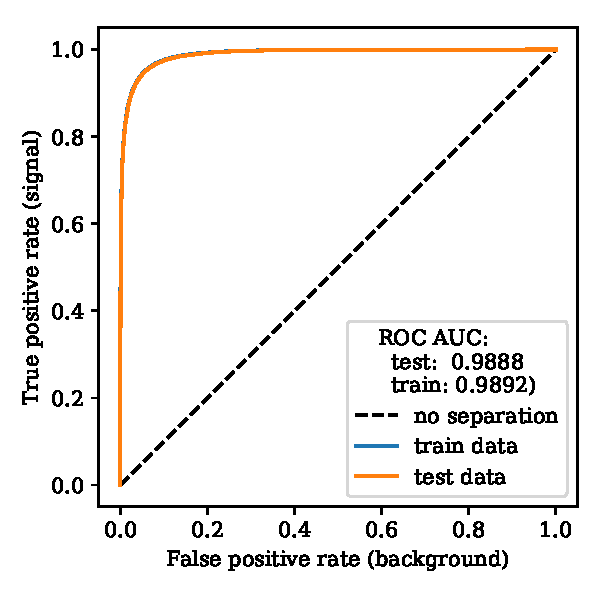
\includegraphics[width=\textwidth]{images/backup/bkg_roc.pdf}
    \end{column}
  \end{columns}
\end{frame}

\begin{frame}{Test on LHCb data: DeepSet output}
  \begin{columns}
    \begin{column}{0.5\textwidth}
      \centering
      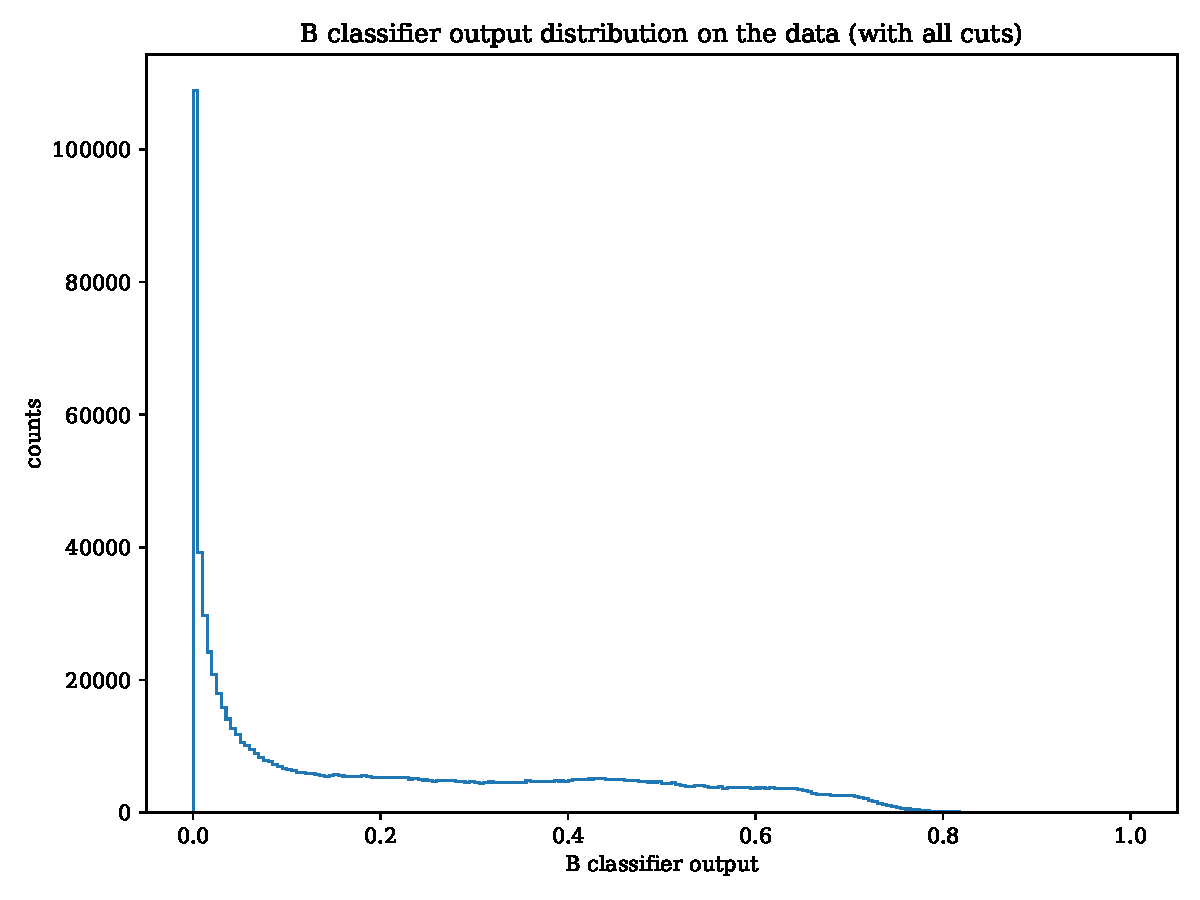
\includegraphics[width=\textwidth]{images/backup/data_B_classifier_output.pdf}
    \end{column}
    \begin{column}{0.5\textwidth}
      \centering
      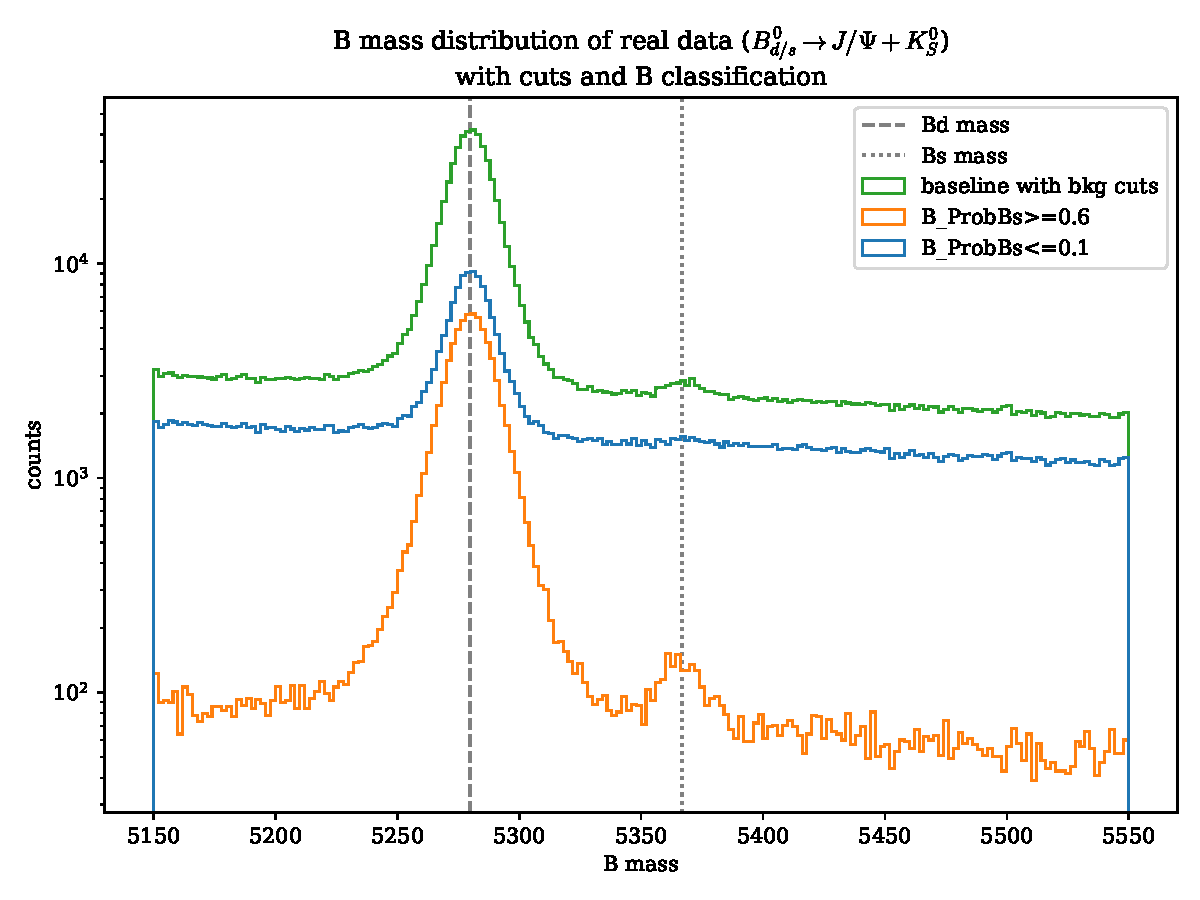
\includegraphics[width=\textwidth]{images/backup/data_cut_comparison.pdf}
    \end{column}
  \end{columns}
\end{frame}

\begin{frame}{Testing on LHCb data: Results (efficiencies, similar to a ROC curve)}
  \begin{columns}
    \begin{column}{0.5\textwidth}
      \centering
      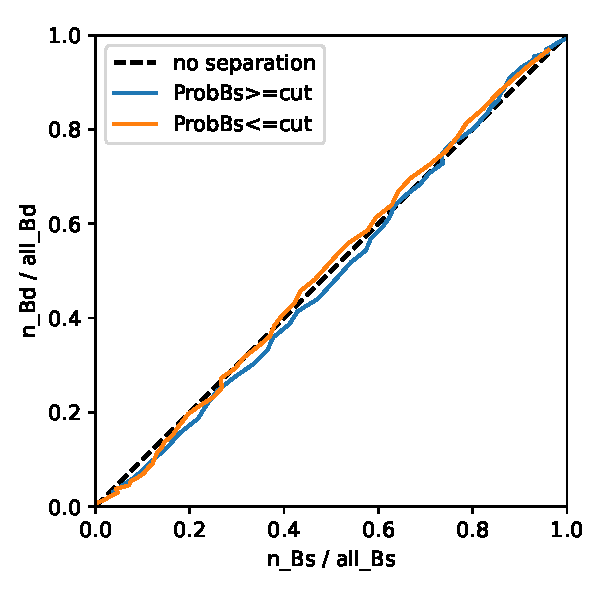
\includegraphics[width=0.9\textwidth]{images/data_roc.pdf}
    \end{column}
    \begin{column}{0.5\textwidth}
      \begin{itemize}
        \item calculated efficiencies $\varepsilon_B = n_B(x)/n_B(\text{no cut})$
        \item plot $\varepsilon_{B_d}$ against $\varepsilon_{B_s}$
        \item should be similar to a ROC curve
        \item no clear separation visible
      \end{itemize}
    \end{column}
  \end{columns}
\end{frame}

\begin{frame}{Fit of the $B_d$ mode on the simulated sample:}
  \centering
  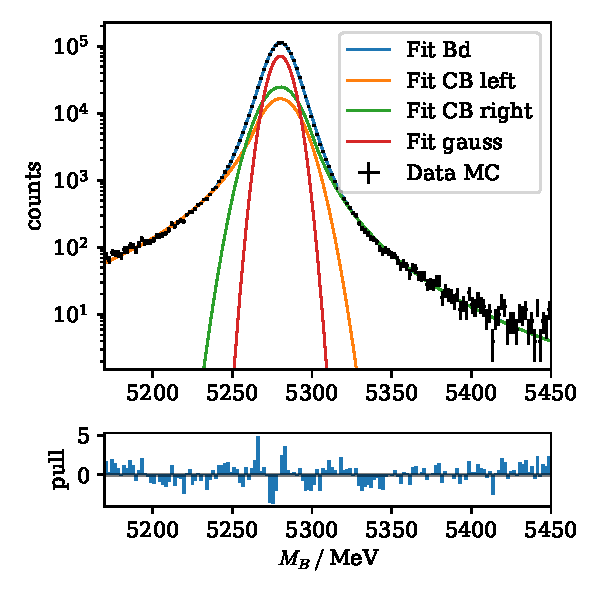
\includegraphics[width=0.5\textwidth]{images/fit_mc.pdf}
\end{frame}

\begin{frame}{Fit functions}
  \begin{equation*}
    F(M_B) = N_\text{bkg} \cdot F_\text{bkg}(M_B) + N_{B_d} \cdot F_{B_d}(M_B) + N_{B_s} \cdot F_{B_s}(M_B)
  \end{equation*}
  \begin{align*}
    F_\text{bkg}(M_B) = \exp(-\lambda \cdot M_B) \, .
  \end{align*}
  \begin{align*}
    F_B(M_B) = &f_1 \cdot f_2 \cdot F_\text{CB}\left(\frac{M_B-\mu}{\sigma_1}, \beta_1, m_1\right) \nonumber\\
                &+ (1-f_1) \cdot f_2 \cdot F_\text{CB}\left(-\frac{M_B-\mu}{\sigma_2}, \beta_2, m_2\right) \nonumber\\
                &+ (1-f_1) \cdot (1-f_2) \cdot F_\text{gauss}\left(M_B,\mu,\sigma_3\right) \, , \label{eqn:FB}
  \end{align*}
  \begin{equation*}
    F_\text{CB}(x,\beta,m) = 
    \begin{cases}
        N \cdot \exp(-\frac{x^2}{2}) & \text{for } x > -\beta \\
        N \cdot \left(\frac{m}{|\beta|}\right)^m \cdot \exp\left(-\frac{\beta^2}{2}\right) \cdot \left(\frac{m}{|b|}-|b| - x\right)^{-m} & \text{for } x \leq -\beta
    \end{cases}
  \end{equation*}
  \begin{equation*}
    F_\text{gauss}\left(x,\mu,\sigma\right) = \frac{1}{\sqrt{2}\pi\sigma} \cdot \exp\left(-\frac{1}{2}\left(\frac{x-\mu}{\sigma}\right)^2\right)
  \end{equation*}
\end{frame}

\begin{frame}{The Standard Model of particle physics}
  \centering
  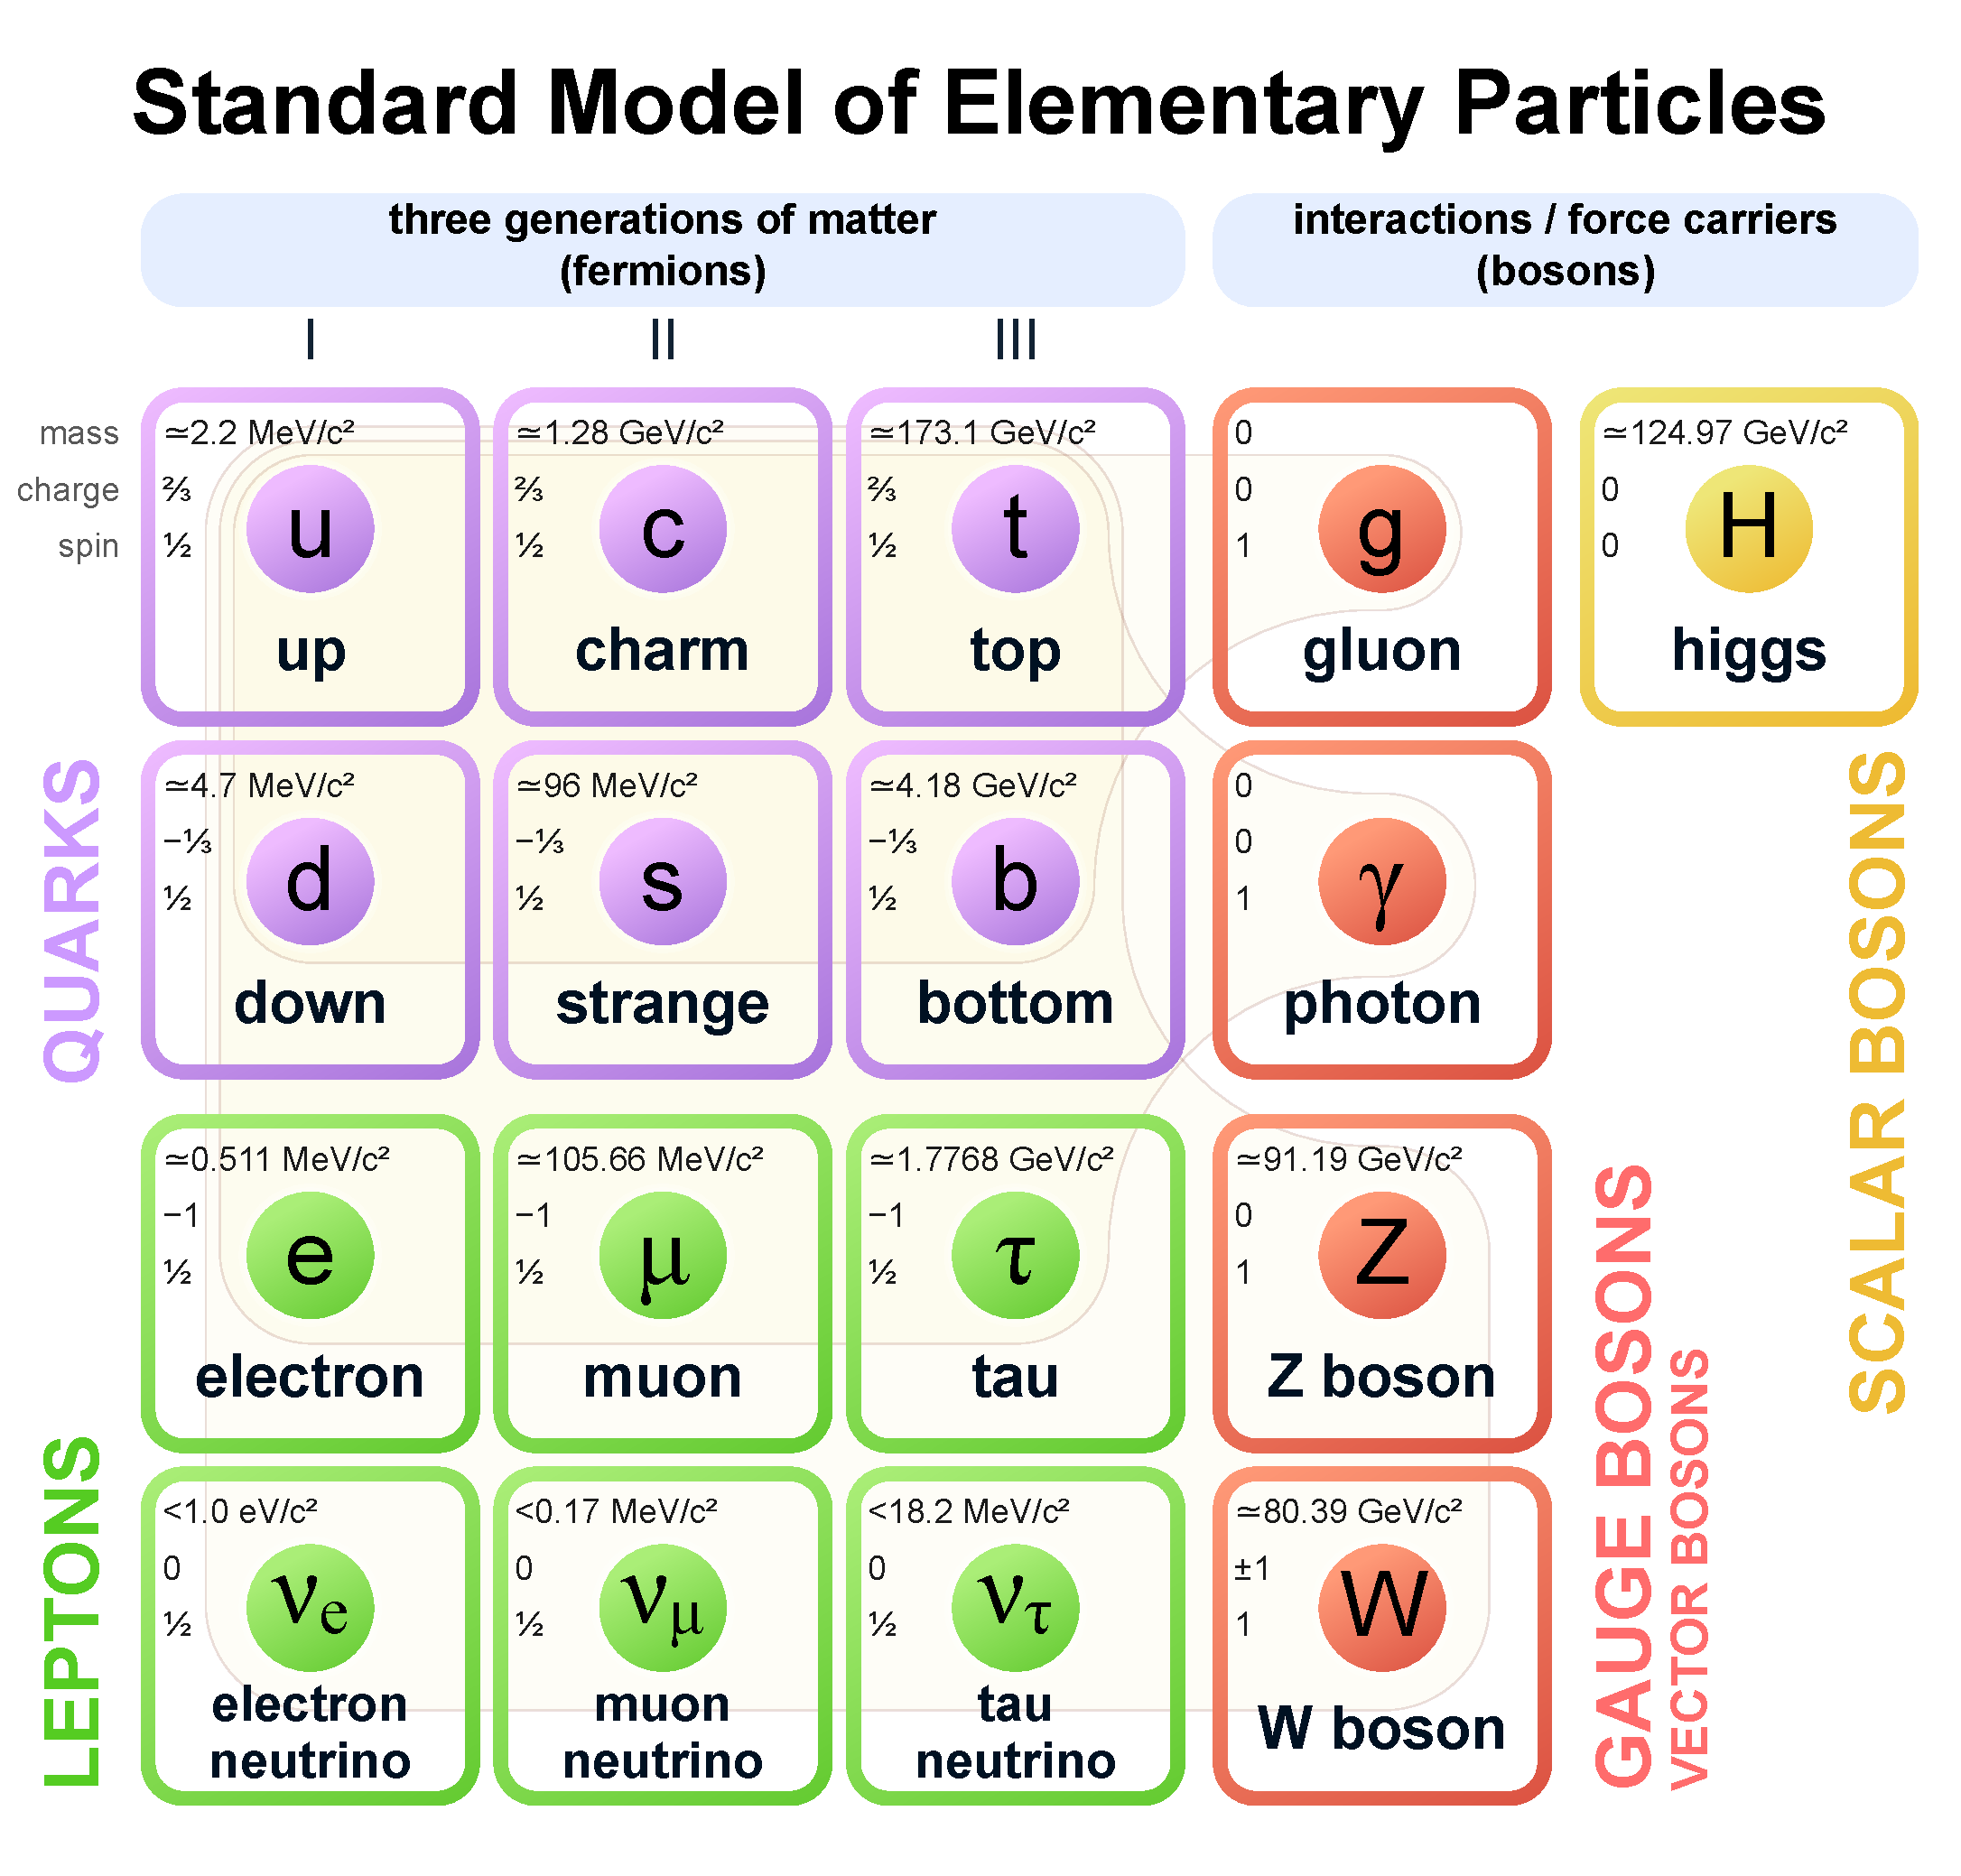
\includegraphics[height=0.9\textheight]{images/standard_model.pdf}

  \tiny \url{https://en.wikipedia.org/wiki/Standard_Model}
\end{frame}

\end{document}